%\documentclass[a4paper,twoside,12pt,dvipdfm]{report}
\documentclass[11pt, a4paper]{report}

\usepackage [shownotes]{101labs}

\addbibresource{101labs.bib}

\coursecode{COMP10120}
\coursename{Introductory Labs}
\title{Lab exercises}
\date{May 2013}
\author{Steve Pettifer, Toby Howard, Graham Gough and John Latham}
\bottomstuff{\noindent
\includegraphics[width=2cm]{images/rpi-logo}\hspace*{\fill}
\includegraphics[width=2cm]{images/Tux}}

\includeonly{rpi1}


\begin{document}


\maketitle
\firstcommand{\tableofcontents\clearpage}


%%% Local Variables: 
%%% mode: latex
%%% End: 

\chapter{Using the School Linux system}

\begin{note}
  This is where the script for the first, one hour lab, should go
\end{note}


Over the next couple of weeks you will be undertaking a number of introductory labs to familiarise yourself with the School's computing infrastructure. Much of this is based on machines running Linux, a variant of the Unix family of operating systems; this document provides some background on Unix and explains why we think it is important. It would very useful if you could read this before you attend the first introductory labs, where the emphasis will be on leading you through a series of tasks to explore our setup.

\section{Operating Systems}

An \wikipedia{Operating_system}{operating system} (OS) is a suite of software that makes
computer hardware usable; it makes the `raw computing power' of the
hardware available to the user. You're probably most familiar with the \wikipedia{Microsoft_windows}{Microsoft Windows} and Apple \wikipedia{OS_X}{OS X} families of operating systems for `desktop' computers, and \wikipedia{Ios}{iOS} (Apple, again) and Google's \wikipedia{Android_(operating_system)}{Android} for mobile devices; but many other more specialist operating systems exist, and you'll be studying some of these and the principles that underpin OS design in COMP25111 in your second year. In the meantime, a potted history of OS development will tide us over\ldots
 
\section{Unix Origins}
\label{sec:unix}


In the late 1950s, an American company called \wikipedia{Bell_Labs}{Bell Laboratories} decided that they needed a system to improve the way they worked with their computer hardware (it's probably quite hard to imagine what interacting with a computer \emph{without} an operating system might be; but it wasn't pretty and involved manually loading and running programs one by one). Together with the \wikipedia{General_Electric_Company}{General Electric Company} and the \wikipedia{MIT}{Massachusetts Institute of Technology}, they set about the design of an operating system they called \wikipedia{Multics}{Multics}: the `Multiplexed Information and Computing Service'. Multics was hugely innovative, and introduced many concepts that we now take for granted in modern operating systems such as the ability for more than one program to run `at once'; but it did rather suffer from `design by committee', and the final system was seen at the time as being overly complex and rather bloated (`bloated' is all a matter of perspective of course: its sobering to realise though that the entire Multics operating system was only around 135Kb. Today's operating systems are something like 30,000 times this size\ldots). In the late 1960s, a group of programmers at Bell Labs created a cut-down, leaner and cleaner version of Multics that would work on more modest hardware. Legend has it that this was to allow them to play their favourite (only!) computer game, \wikipedia{Space_Travel_(video_game)}{Space Travel}. In an early example of the trend of giving things `punny' names, to contrast with the more clumsy Multics, they called this new system Unix. The so-called \wikipedia{Jargon_File}{Jargon File} is a good source of explanations of various bits of computer slang and their obscure origins, and is well worth a read: in part to give some background history, but mostly as an insight into the minds of the computing pioneers of the past!

%\begin{htmlonly}
%(See the Unix entry in the useful and amusing
%\htmladdnormallink{Jargon
%file}{http://www.new.ox.ac.uk/admin/jargon/html/entry/Unix.html}, a
%file}{http://www.cs.manchester.ac.uk/software/jargon/html/entry/Unix.html}, a
%file}{\jargonFileUnix}, a
%`collection of slang terms used by various subcultures of computer
%\htmladdnormallink{hackers}
%{http://www.cs.manchester.ac.uk/software/jargon/html/entry/hacker.html}'.)
%{\jargonFileHackers}'.)
%\end{htmlonly}

Even though Unix is now quite old, most Computer Scientists recognise that the designers of Unix got most of the fundamental concepts and
architecture right. Given how much computing has changed since the 1960s, this was an astonishing intellectual achievement. Although Microsoft's \wikipedia{Microsoft_Windows}{Windows} is by far the most common operating system on \emph{desktop} machines, the majority of the Internet, much of the world's corporate infrastructure, virtually all supercomputers, and even some mobile devices are powered by Unix-like operating systems. So, while the polished graphical user interfaces of Windows and \wikipedia{OS_X}{OS X} appear to dominate the world of computing, most of the real hard-core and leading-edge computation relies on an elegant operating system designed nearly 50 years ago (by a team of scientists who wanted to play a game).  

\section{Modern Unix Variants}
\label{sec:modern-unix-variants}


The history of Unix is complex and convoluted, with the system being updated, re-implemented, and mimicked repeatedly over the years, primarily by commercial companies who guarded their versions jealously. Figure \ref{fig:unix-history} shows a tiny fragment of the Unix's `family tree' (the full diagram, which you can find at \url{http://www.levenez.com/unix/unix.pdf}, is \emph{many} times the size of the portion you can see here).

\begin{figure}[h!tb]
  \begin{center}
    \includegraphics[width=13cm]{images/unix}
  \end{center}
\caption{A fragment of \'{E}ric L\'{e}v\'{e}nez's Unix History chart, reproduced with permission and showing the beginnings of Linux in amongst other versions of Unix.}
\label{fig:unix-history}
\end{figure}
 
Although many of the branches represent interesting innovations of one kind or another, there are perhaps two that deserve particular attention. The first of these was the decision by Apple some time around the turn of the millenium to drop their own---highly popular, but aging---bespoke operating system (unimaginatively called \wikipedia{Mac_os_9}{Mac OS 9}) in favour of a Unix-based system (now the more familiar `OS X', where `X' is both the Roman numeral `10' and a nod in the direction of the uniX nature of the OS). Although the majority of Mac users are blissfully unware of the fact, behind the slick front-end of OS X, sits a variant of Unix. The second, and perhaps more profound of these events was the creation in 1991 by Swedish programmer \wikipedia{Linus_torvalds}{Linus Torvalds} of a Unix-like system, the source code to which \emph{he gave away for free}\footnote{`free' here in the sense both of `freedom to reuse or adapt', and also in the sense of `without charge'.}; this became known as the \wikipedia{Linux_kernel}{Linux Kernel}. Combined with other free software created by the \wikipedia{Free_software_foundation}{Free Software Foundation}, a non-commercial version of Unix called \wikipedia{GNU/Linux}{GNU/Linux} was born (GNU here is a recursive acronym for ``GNU's not Unix'', a swipe at other commercial non-Free versions; much to the annoyance of the Free Software Foundation, GNU/Linux is almost always called just `Linux'\footnote{Linux
is pronounced ``Linn-ucks'', despite the fact the name was coined by
its creator, and his name `Linus' is pronounced
``Leen-uss''!}.) 

Linux has been, and continues to be, developed cooperatively by
thousands of programmers across the world contributing their effort
largely free of charge. It is amazing to think that such
a project could ever happen---and it is surely a testament to the
better side of Human nature. But what is interesting is the
observation that these programmers are not motivated by commercial
concerns, but by the desire to make good reliable software and have it
used by lots of people. Thus, Linux is a good choice of Unix: it's
Free, it's efficient, and it's reliable, and it is now used by large corporations, governments, research labs and individuals around the world. Even Google's \wikipedia{Android_(operating_system)}{Android} platform is a Linux-based mobile OS, and the  \wikipedia{Amazon_Kindle}{Amazon Kindle} is also a Linux box behind its user interface.

One of the results of the fact that Linux is Free is that several
organisations and companies have created their own distributions of
it; these vary a bit (in fact, anybody is free to make any change they
like to Linux, and pass it on to whoever wants it). The distribution
we use in this School is \textbf{Fedora}, which is
one of the most popular and is sponsored by a
US company called \textbf{Red Hat}.
%, which is the latest release

So, if you are to become an expert computer professional, it is
important that you understand the theory and practice of Unix based
systems. Learning Unix is not only a crucial skill for any serious
computer scientist, it is a very rewarding experience; the labs over
the next couple of weeks are designed to help you become familiar with what will be your daily working environment.


` \chapter{Getting started with Raspberry Pi}

% TODO: Intro to what they have been given, and labelling their Pi
% TODO: References, references.
% TODO: Wikipedia links
% TODO: The Pi is yours to keep; if you lose it you'll have to buy another
% TODO: What you'll need to use the Pi at home
% TODO: Where do we introduce 'devices', 'files' and 'processes'? They will see virtual devices like tty0 and sda1 

The Raspberry Pi is an astonishing piece of hardware. Not because it is super-fast or super-powerful---it's actually quite a slow computer by today's standards---but because it is small, cheap and needs very little energy to run. Its cheapness means you can experiment with it safe in the knowledge that if you mess it up, lose it, or drop it into the canal, getting hold of a replacement isn't going to cost you much more than a text-book or a night out at the cinema. Its small size and fairly modest power requirements mean you can be put to use in lots of applications where a regular-sized PC would be impractical.  We hope this will encourage you to experiment and explore, and to take risks playing with both its hardware and software that you might be reluctant to do on your own computer or tablet, or simply can't do with the School's lab machines. 

This lab session is designed to get you familiar with the Raspberry Pi itself, and with some of the basics of the Linux operating system it uses. We're going to be covering a lot of ground quite quickly, and it's important that you read these notes carefully and follow the instructions precisely for now. As the lab sessions progress, the instructions will become much less prescriptive, and we'll be encouraging you to experiment and explore much more, and to find out things for yourself. But for now, just follow our lead. 

Scattered throughout the main text of these exercises there are information boxes of various kinds:
\\

\begin{tabular}{m{1.5cm}m{12cm}}
{
\includegraphics[width=1.5cm]{images/bomb}} & \textbf{Danger!} The bomb icon explains problems and pitfalls, and how to avoid them. It's really important that you read these sections, or you may regret it later.\\
\\

\includegraphics[width=1.5cm]{images/rpi-logo} & \textbf{Raspberry Pi Facts and Factoids.} These sections explain useful but non-essential things about the Raspberry Pi. If you're pushed for time, you can safely skip these boxes and perhaps come back to them another time.\\
\\

\includegraphics[width=1.5cm]{images/diversion} & \textbf{We digress\ldots} Boxes marked with this icon contain digressions and facts that are hopefully interesting but are probably tangential to the main flow of the exercise.\\
\end{tabular}

\FloatBarrier 
\section{The Raspberry Pi}

The most remarkable thing about the Pi is that, although it's a bit underpowered in many ways, it is capable of running the same full Linux Operating System as the machines that you'll be using in the labs for the duration of your studies, and which you'll undoubtedly encounter in your future careers. Actually we're going to be using slightly different flavours of Linux on the Pi and the lab machines, but the differences are fairly minor---more on that later. Let's get started. 

The Raspberry Pi itself is just the circuit board shown from the top in Figure \ref{figure:bare-rpi}. The case we've put yours in is clear plastic so you can see the Pi inside, but you're welcome to change it for another style if you prefer (there are plenty available to buy online, and lots of people have made their own unique ones just for the fun of it). The Pi is reasonably robust, and you can use it without a case, but obviously it's a bit more vulnerable if its not in a box of some sort. Figure \ref{figure:bare-rpi-underside} shows the Pi's circuit board from beneath, with an SD card inserted.

\begin{rpi}{Why Pi?}
  The Raspberry Pi apparently got its name because (a) lots of other computer systems have been named after fruit (you'll know of Apple and Blackberry, but in the past there has also been at least Apricot and Tangerine), and (b) the \wikipedia{Python_(programming_language)}{Python language} was one of the first things ported to run on it. The logo was created by Paul Beech, and is based on Buckminsterfullerene, a spherical fullerene molecule more commonly called a Buckyball. Its designer pointed out that a full buckyball has 32 faces, but that only 11 are visible in the 2D logo; and that the Raspberry Pi has a 32-bit processor and an ARM11 on board.

The ARM processor, on which the Pi and the vast majority of the world's other mobile devices are based, was originally designed by a team led by \wikipedia{Steve_Furber}{Steve Furber}, who is a Professor in this School.  
\end{rpi}

\begin{figure}
\centerline{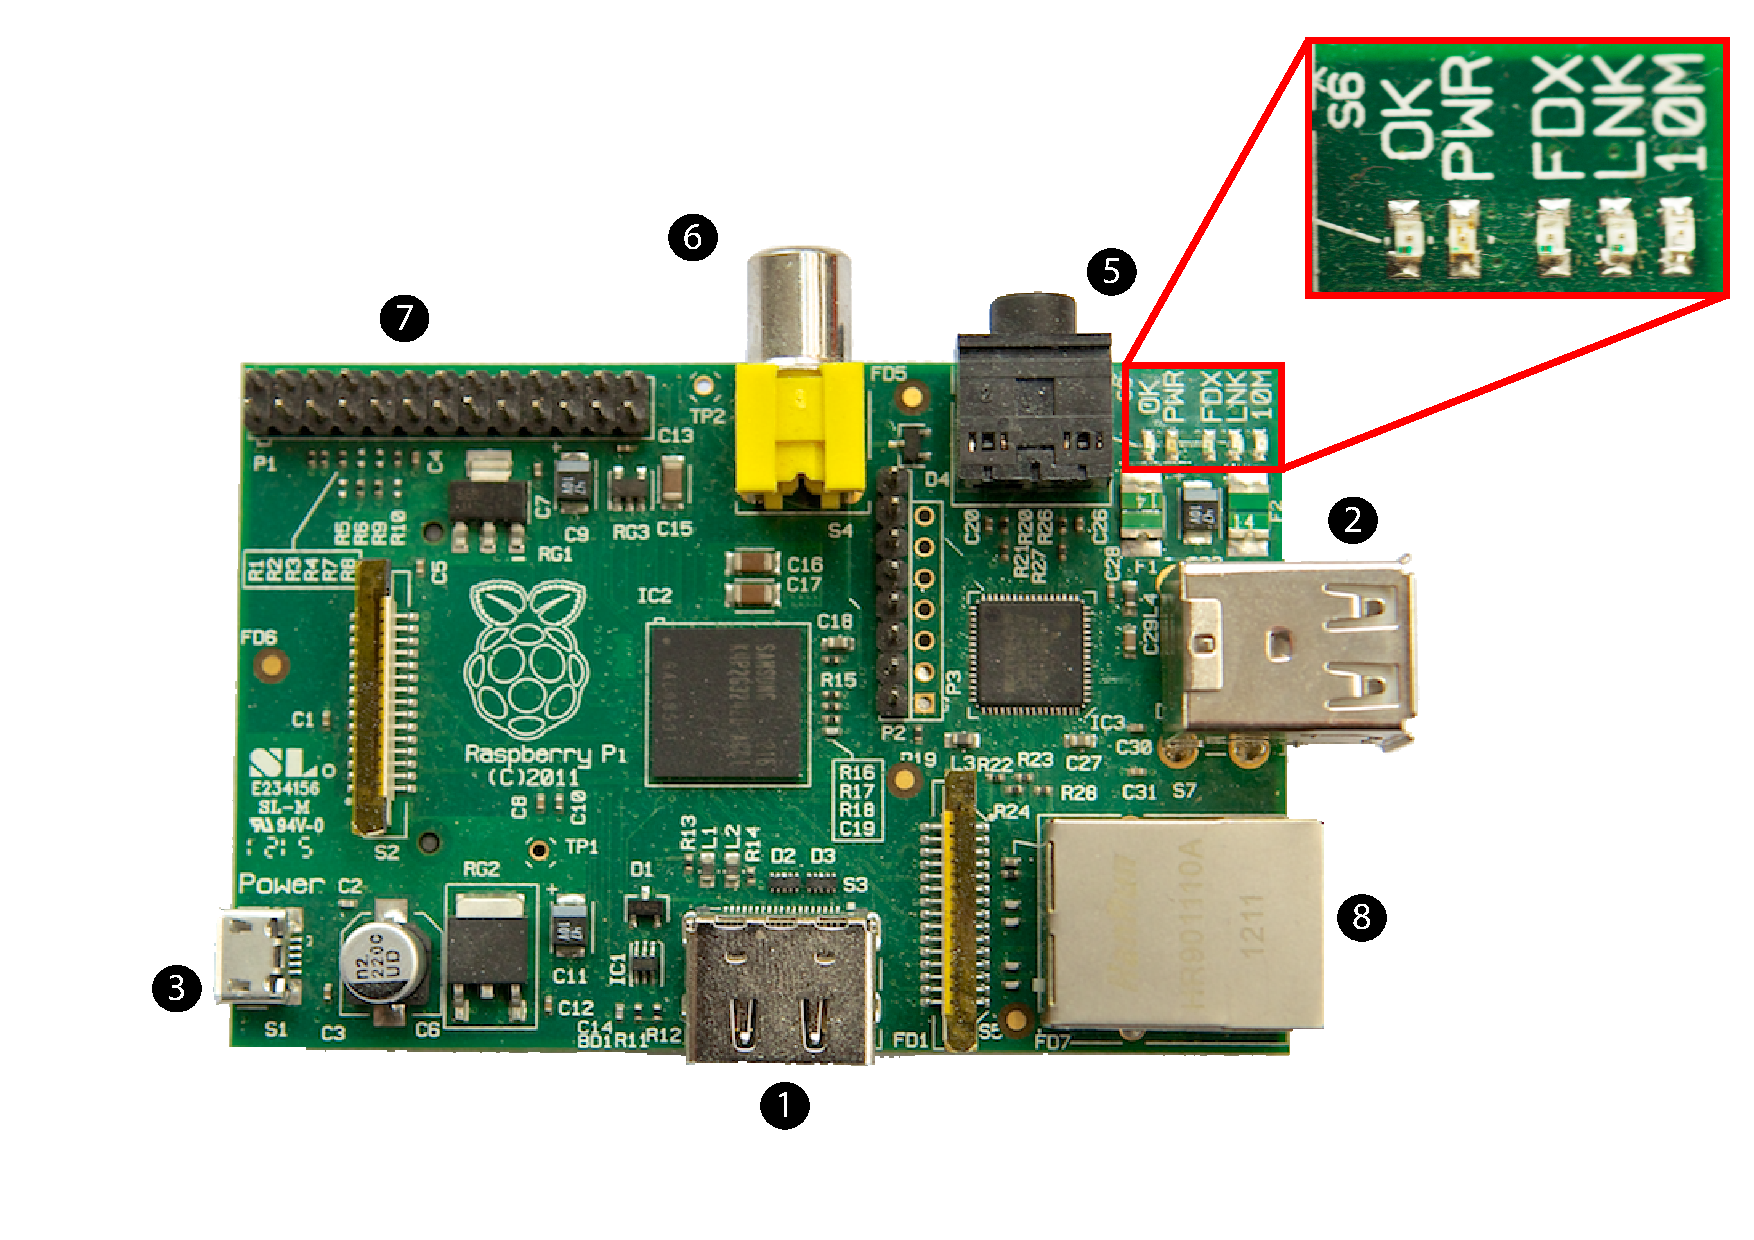
\includegraphics[width=15cm]{images/bare-rpi-annotated}}
\caption{An uncased Raspberry Pi, and an expanded view of the indicator LEDs at the board's top right. The numbered connectors are \protect\circled{1} HDMI output,  \protect\circled{2} USB,  \protect\circled{3} power,  \protect\circled{5} audio output,  \protect\circled{6} composite video out,  \protect\circled{7} General Purpose Input/Output (GPIO),  \protect\circled{8} Ethernet.}\label{figure:bare-rpi}
\end{figure}

\begin{figure}
\centerline{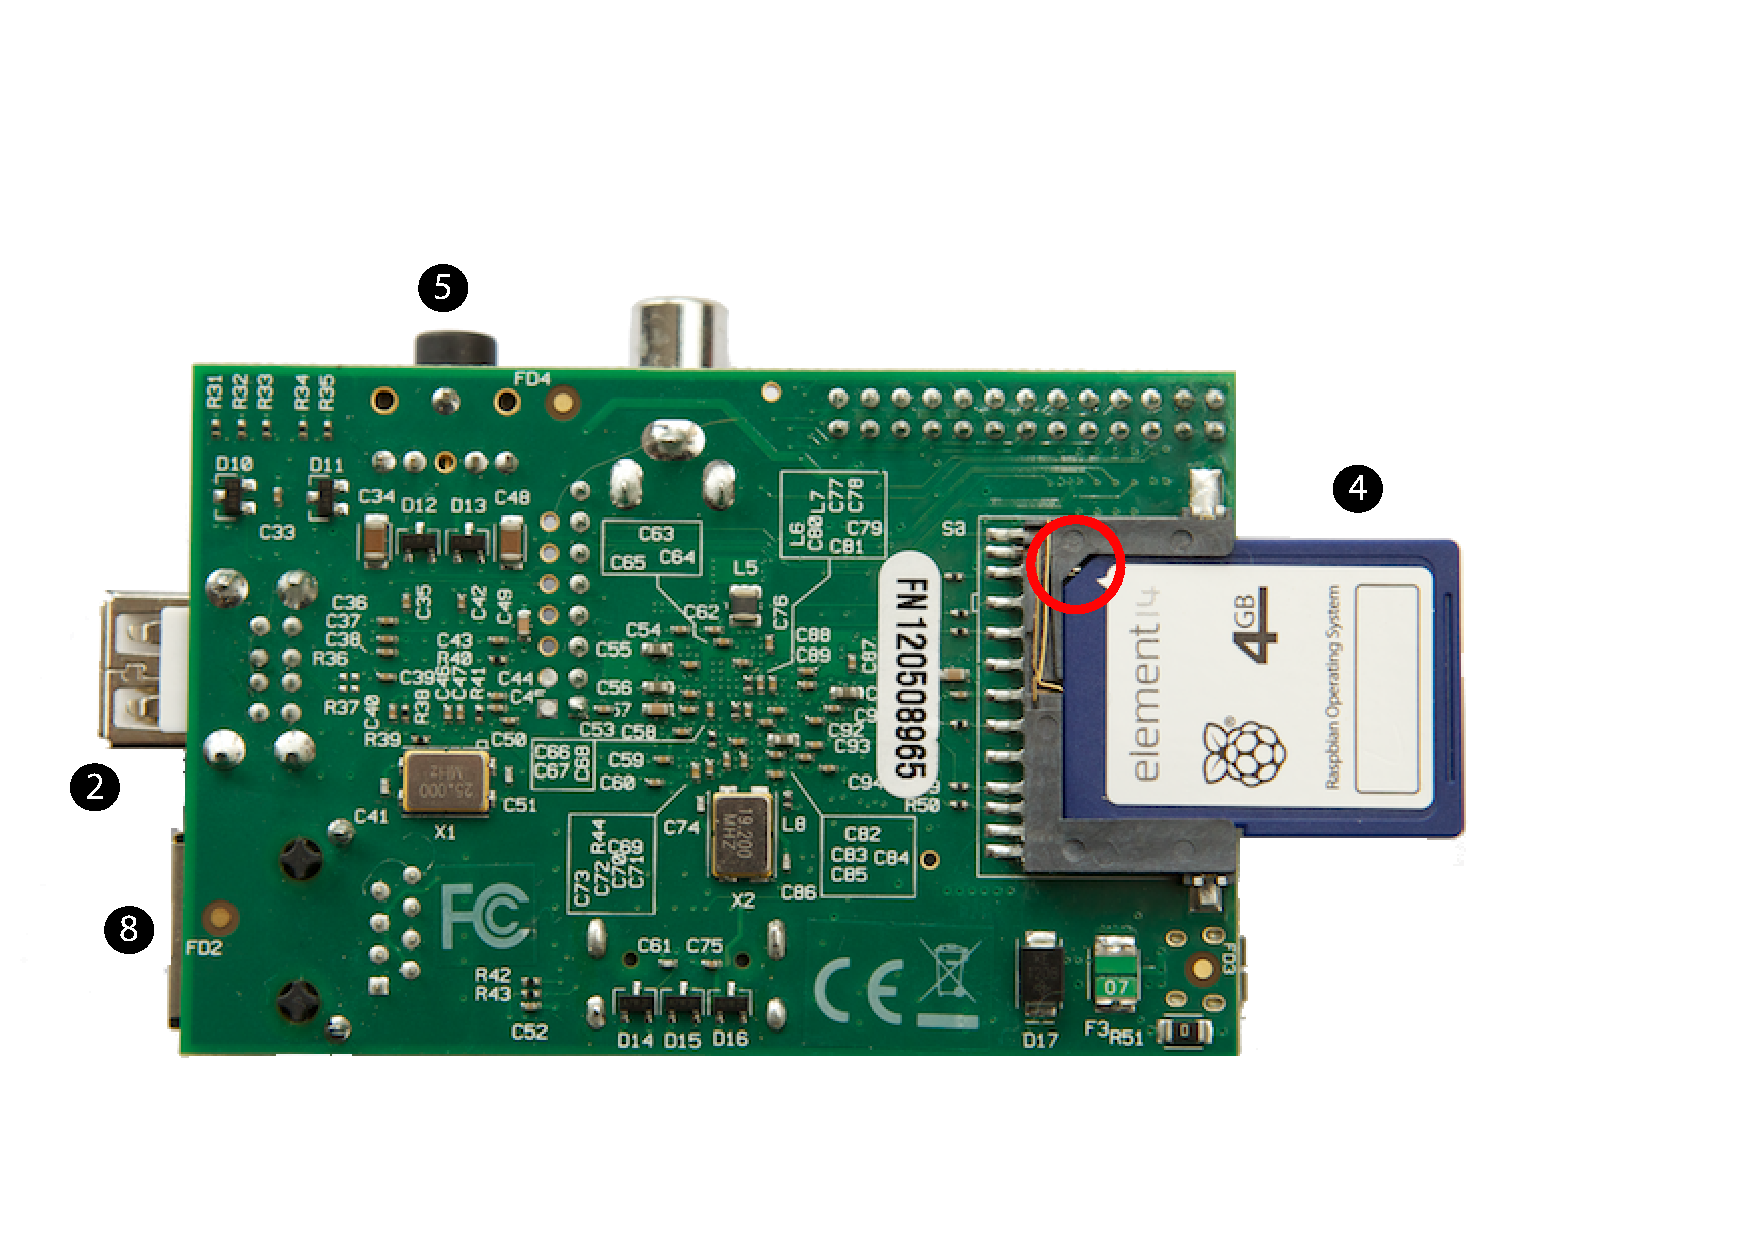
\includegraphics[width=15cm]{images/bare-rpi-underside-annotated}}
\caption{A naked Raspberry Pi. The circle indicates the location of the bevelled corner to orient the card. The ports are numbered as in Figure~\ref{figure:bare-rpi}, and in addition \protect\circled{4} shows the location of the SD (Secure Digital) memory card. The red circle indicates the locating bevel on the card.}\label{figure:bare-rpi-underside}
\end{figure}

It's important that you connect the Pi up in exactly the order specified here---so even if you are familiar with using a Pi, please don't jump ahead and plug everything in at once (no harm will come to the Pi if you do, but this exercise relies on your following our instructions closely). The monitors in the LF31 Lab are all fitted with an extra video lead for connecting up the Pis. Locate the HDMI lead, and plug this into the socket marked \circled{1} on Figure~\ref{figure:bare-rpi}. Next we'll need to connect a keyboard. Follow the cable that comes out the back of the keyboard towards where it vanishes into the desk, and you'll see an inline USB connector that will allow you to unplug the keyboard from the desktop PC and into one of the two USB sockets on your Pi; these are marked with \circled{2} on the Figure. It doesn't matter which USB socket you choose, but please make sure to reconnect this to the PC when you're done with these experiments, just as a courtesy to the next user. 

Next, we need to insert the \wikipedia{Secure_Digital}{Secure Digital} (SD) card that contains the Pi's operating system, and on which you'll be storing your own files. Look at Figure ~\ref{figure:bare-rpi-underside}, make sure the SD card is orientated correctly (note the position of the little cut corner) and gently push it into the socket; around half of the card will remain protruding outside the case. \textbf{Don't} plug a mouse in at this stage; you won't need it until the very last part of the exercise.

\begin{rpi}{Raspbian}
  The SD card we've provided for you has already had the standard Raspbian version of Linux written onto it (it's a version of the Debian release of Linux, tuned for the Pi). If you do manage to corrupt the operating system, or just want to start from scratch, then re-writing the SD card with a fresh image is reasonably straightforward: there are plenty of instructions online on how to do this, and we've provided you with a USB multi-card reader/writer that you can use for the job. The process does require access to what's called the `raw' device though, and on Linux that requires administrator access to the machine, so you'll have to use your home machine or someone else's Raspberry Pi to do this.

  Instructions on how to get hold of the files you'll need, and how to write them to the SD card on various operating systems are available at \url{http://www.raspberrypi.org/downloads}. You might want to think about getting a larger SD card in any case; the one we've given you is fine for the labwork we've set, but probably a bit on the small side for anything else. SD cards are widely available in shops and online, and aren't expensive. But you should check whether the specific card you're going to buy is compatible with the Pi before parting with any money---differences in the read/write speeds of some cards mean they don't play nicely with the Pi.
\end{rpi}

Now you're ready to power up the Pi. From the back of the monitor you'll notice a Micro USB cable (the same connector that you'll find on many modern smartphones and tablet devices). This goes into the socket marked \circled{3} on Figure \ref{figure:bare-rpi}. There is no power switch on the Pi, so as soon as the power cable goes in, it will start to boot (this strange term is explained in breakout box~\ref{boot box}): the red PWR LED should light up and stay on, and you'll also notice that the OK LED (which indicates SD-card activity) to its left also flickers. If any of the other three LEDs marked FDX, LNK, or 10M are lit, then that means you've already plugged a network cable into your Pi, in which case please unplug that now!

\begin{danger}{Pi Power} 
Like most other computers, the Pi doesn't like having its power removed without being shut down properly. Although you might get away with it, there's a reasonable chance of messing up the operating system if you remove the power while the Pi is in the middle of doing something. And because the Pi runs a multi-tasking operating system, it's almost always `doing something', so pulling the power out unexpectedly is always a bad idea. You're unlikely to damage the Pi's hardware like this, but you may find that you lose work, and may have to reinstall the operating system. For instructions on how to shut the Pi down safely, see Section \ref{section:shutdown}.
\end{danger}

Refer to Figure~\ref{figure:monitorswitch} and switch the Input Selection on the monitor from VGA (which is the input used by the PC under the desk) to DVI (the cable you've connected your Pi to is a HDMI to DVI cable), and all being well you should see a black screen containing the Raspberry Pi logo at the top left, and white text that scrolls up the screen as the Pi boots. When the boot process finishes for the first time (it will take somewhere about 20--30 seconds), if all has gone well you should see the Pi's configuration tool appear (see Figure \ref{figure:raspi-config}).

% TODO: needs a photo of the monitor / switch here
\begin{figure}
\centerline{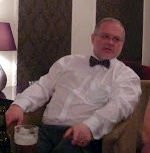
\includegraphics[width=5cm]{images/mysteryimage}}
\caption{The Input Selection switch on the monitor.}\label{figure:monitorswitch}
\end{figure}

\begin{diversion}{Booting}
\label{bootbox}
The phrase `booting' to refer to the process of starting up some computer system has become quite commonplace, but its origins are rather strange. It's thought to have first been used in early 19th Century America as a way of describing an obviously impossible action such as to ``pull onself over a fence by one's bootstraps''. These days it is used to refer to any self-sustaining process that is able to happen without external help. 

So why is starting a computer a bootstrapping process? In order for you as a user to be able to run a program, the computer needs an operating system. But in order to load its operating system, it needs some instructions that tell it how to understand the file system. And in order to load the instructions that tell it how to understand the file system it needs to\ldots well, you get the idea. In reality, most computers have a very small set of instructions hardwired into them that begin the process of loading a  slightly more complex `bootloader', which then begins the process of loading the OS kernel and any modules needed to interact with the hardware, and then starts loading services and features of increasing sophistication that rely on the simpler ones loaded previously to function. 

As an aside, you want to consider this: if you need a text editor to write programs, how did the first text editor (which is itself a program) get written?
\end{diversion}

\begin{figure}
\centerline{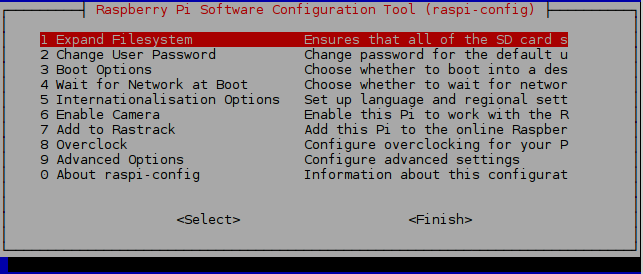
\includegraphics[width=13cm]{images/raspi-config.png}}
\caption{The Raspberry Pi config tool. The highlight bar can be moved between the different controls using the Tab key, or up and down in the menu using cursor keys.}\label{figure:raspi-config}
\end{figure}

Before using the Pi for real, you'll need to perform one task using this menu. Use the up and down cursor keys to move the selection bar to the \ttout{expand\_rootfs} option, and press Enter. You'll see a confirmation that `Root partition has been resized. The filesystem will be enlarged upon the next reboot'. If that doesn't mean anything much to you right now, don't worry, we'll come back to an explanation of that later (see Section~\ref{section:expandfs}). For now just press Enter again to get back to the main menu. 

At this stage you could tweak various other options that affect the display and the layout of keyboard being used; but conveniently the defaults set on the Pi will do just fine for now (it is a mostly British invention after all, so it defaults to UK keyboard layout!) Use the Tab key to move the red highlight to \ttout{<Finish>}, and hit Enter again. The Pi will reboot (an example of what this looks like is shown in Figure \ref{figure:piboot}) and this time when the process finishes you'll be presented by a UNIX login prompt which will say something like:

\begin{figure}
\centerline{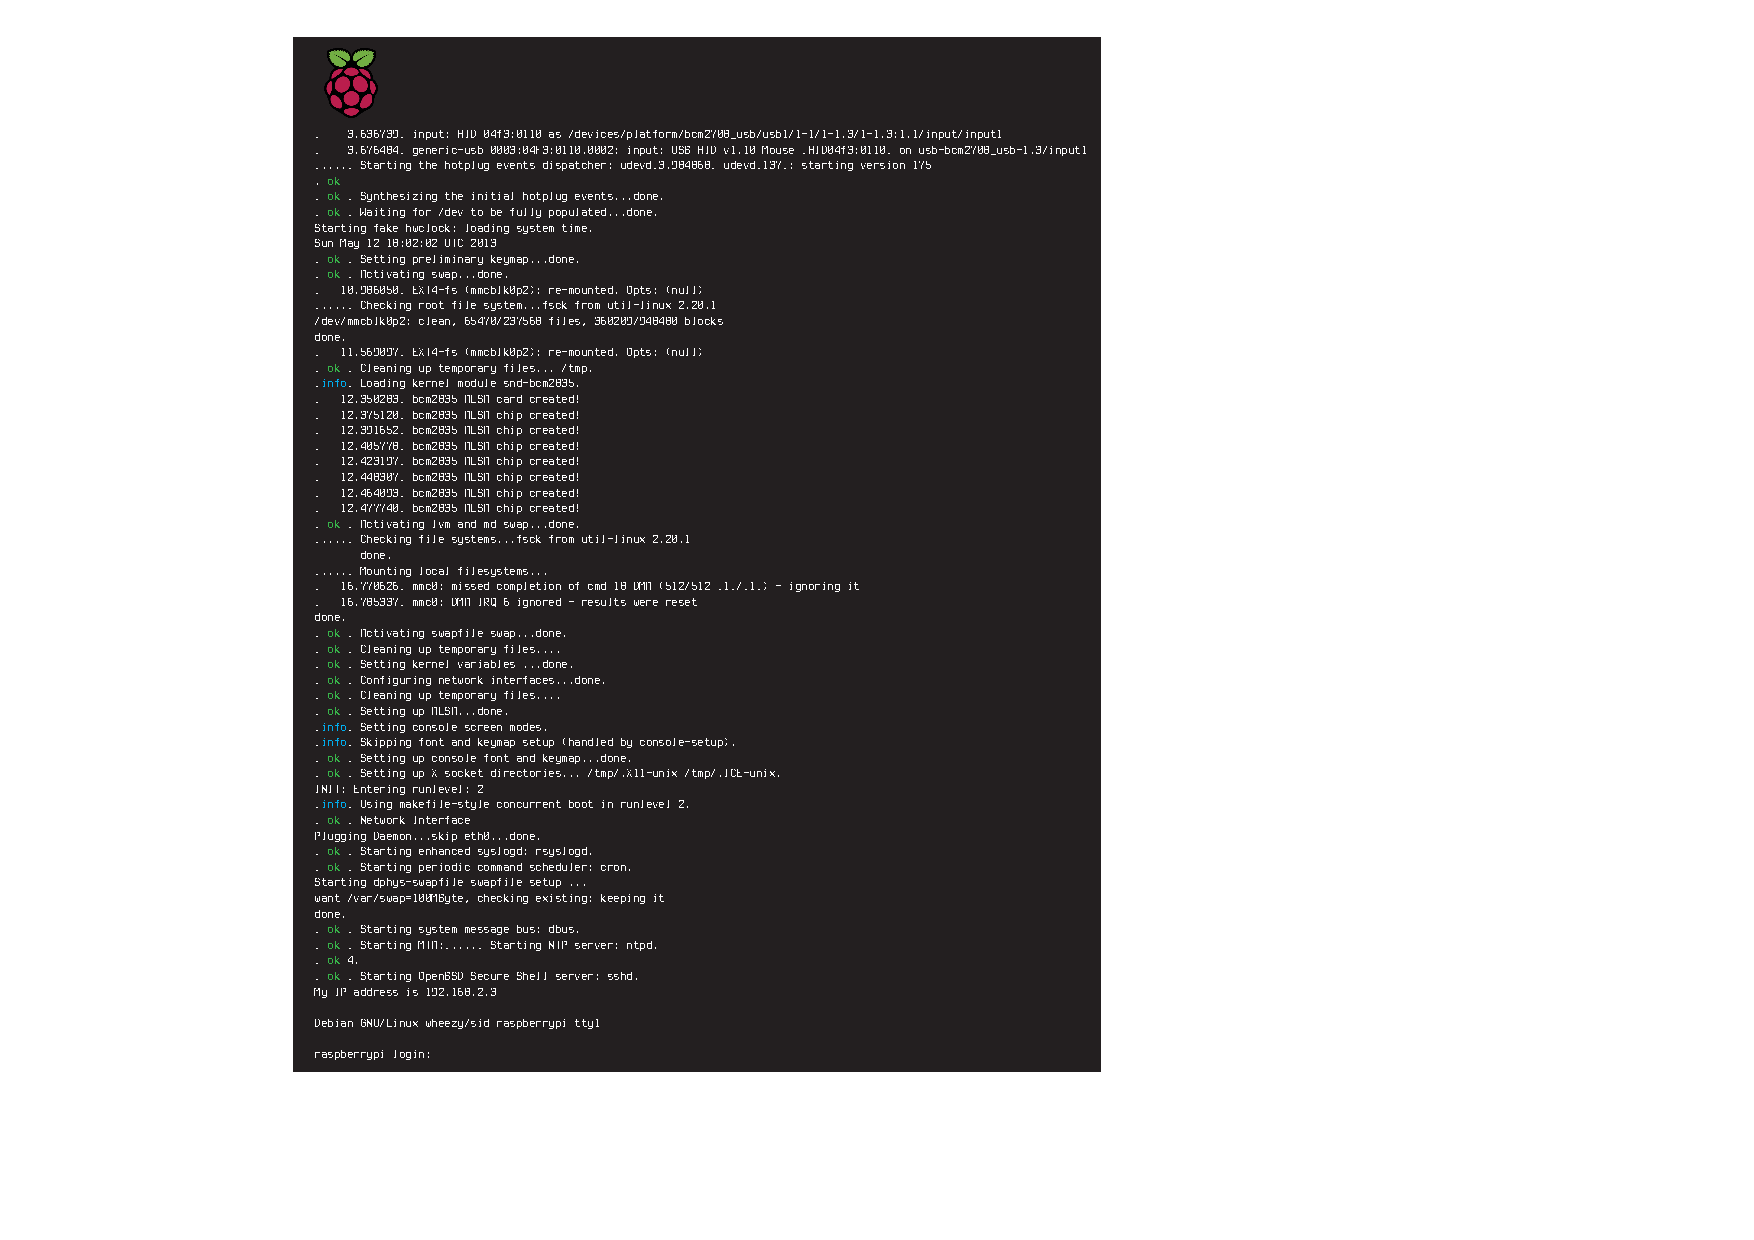
\includegraphics[width=15cm]{images/bootscreen}}
\caption{A sample Raspberry Pi bootscreen. The exact layout and details may vary depending on the size/shape of the screen and the configuration of the Pi.}\label{figure:piboot}
\end{figure}

\begin{ttoutenv}
Debian GNU/Linux wheezy/sid raspberrypi tty1

raspberrypi login:
\end{ttoutenv}

At the login line enter \totype{pi} as the username, and when prompted for the password, type \totype{raspberry}. \textbf{Note that the username will appear on screen as you type it, but the password will not} (so make sure you're typing carefully!) You should see:

\lstset{moredelim=[is][\textbf]{|}{|}}
\begin{lstlisting}
Last login: Mon Feb 16 14:46:27 2015
Linux raspberrypi 3.18.7-v7+ #755 SMP PREEMPT Thu Feb 12 17:20:48 GMT 2015 armv7l

The programs included with the Debian GNU/Linux system are free software;
the exact distribution terms for each program are described in the
individual files in /usr/share/doc/*/copyright.

Debian GNU/Linux comes with ABSOLUTELY NO WARRANTY, to the extent
permitted by applicable law.
|pi@raspberrypi ~ $|
\end{lstlisting}


%

The last line of this text (which is shown in bold here but will be green and blue on your screen) is the command prompt. It might look innocent enough, but in the right hands, the command prompt is one of the most powerful ways of controlling a computer. It may feel a bit odd at first if you're used to a graphical interface, but being comfortable with issuing instructions to a machine via a textual command-line rather is a crucial skill that you'll need during your studies here at University, and also in your future career.

\begin{diversion}{Don't be a WIMP}
The familiar Windows, Icons, Menus and Pointer (WIMP) paradigm used on most graphical desktop environments is enormously powerful, but it's not suitable for every task, and understanding when you're better off using the command-line or a keyboard shortcut instead will make you a lot more efficient.

Sometimes the clumisness of the GUI comes from the fact that there's no convenient visual metaphor for a particular action; how do you graphically represent the concept of `rename all the files I created yesterday so they start with a capital letter'? 

But a lot of the time the issue is simply that it takes much longer to do some things with the mouse than it does with a keystroke or two. Every time you use the mouse, a little time is wasted shifting your hand off the keyboard and a little more time used up tracking the pointer between the on-screen widgets. For casual use, this wasted time really doesn't matter. But as a computer scientist you're going to be spending a lot of time time in front of a machine, and all the seconds wasted moving the mouse pointer around add up. 

What's really fascinating here, though, is that although the keyboard versus mouse debate is one that has been running for at least the mid-1980s, there isn't a clear winner, or even any definitive guidelines as to when one is better than the other. 

In any case, you should definitely learn the keyboard shortcuts for the most common operations in your favourite tools, and a handful of useful command-line tools. For example, when you're writing code you'll be saving files very regularly; maybe even several times a minute when you're debugging. There are two options for this: 1) move hand off keyboard to mouse; use pointer to find the `File' menu, from the file menu move the pointer to the `Save' option; move hand from mouse back to keyboard. Or 2) Press the combination of keys that perform the `save' function. Which do you think is faster?

And think carefully about the best tool for the job; sometimes it'll be the mouse/menu combination, but perhaps more often than you might think, a few selected commands may get the job done considerably more quickly. In particular, you've probably had more experience of doing things the GUI-way up until now, so if it's not obvious which is the better choice for a particular task, we suggest you go for the command-line option until you're familiar enough with the pros and cons of both approaches to make an informed decision each time.
\end{diversion}

The default command prompt on the Pi consists of four components shown in Figure \ref{figure:prompt}.

\begin{figure}
\centerline{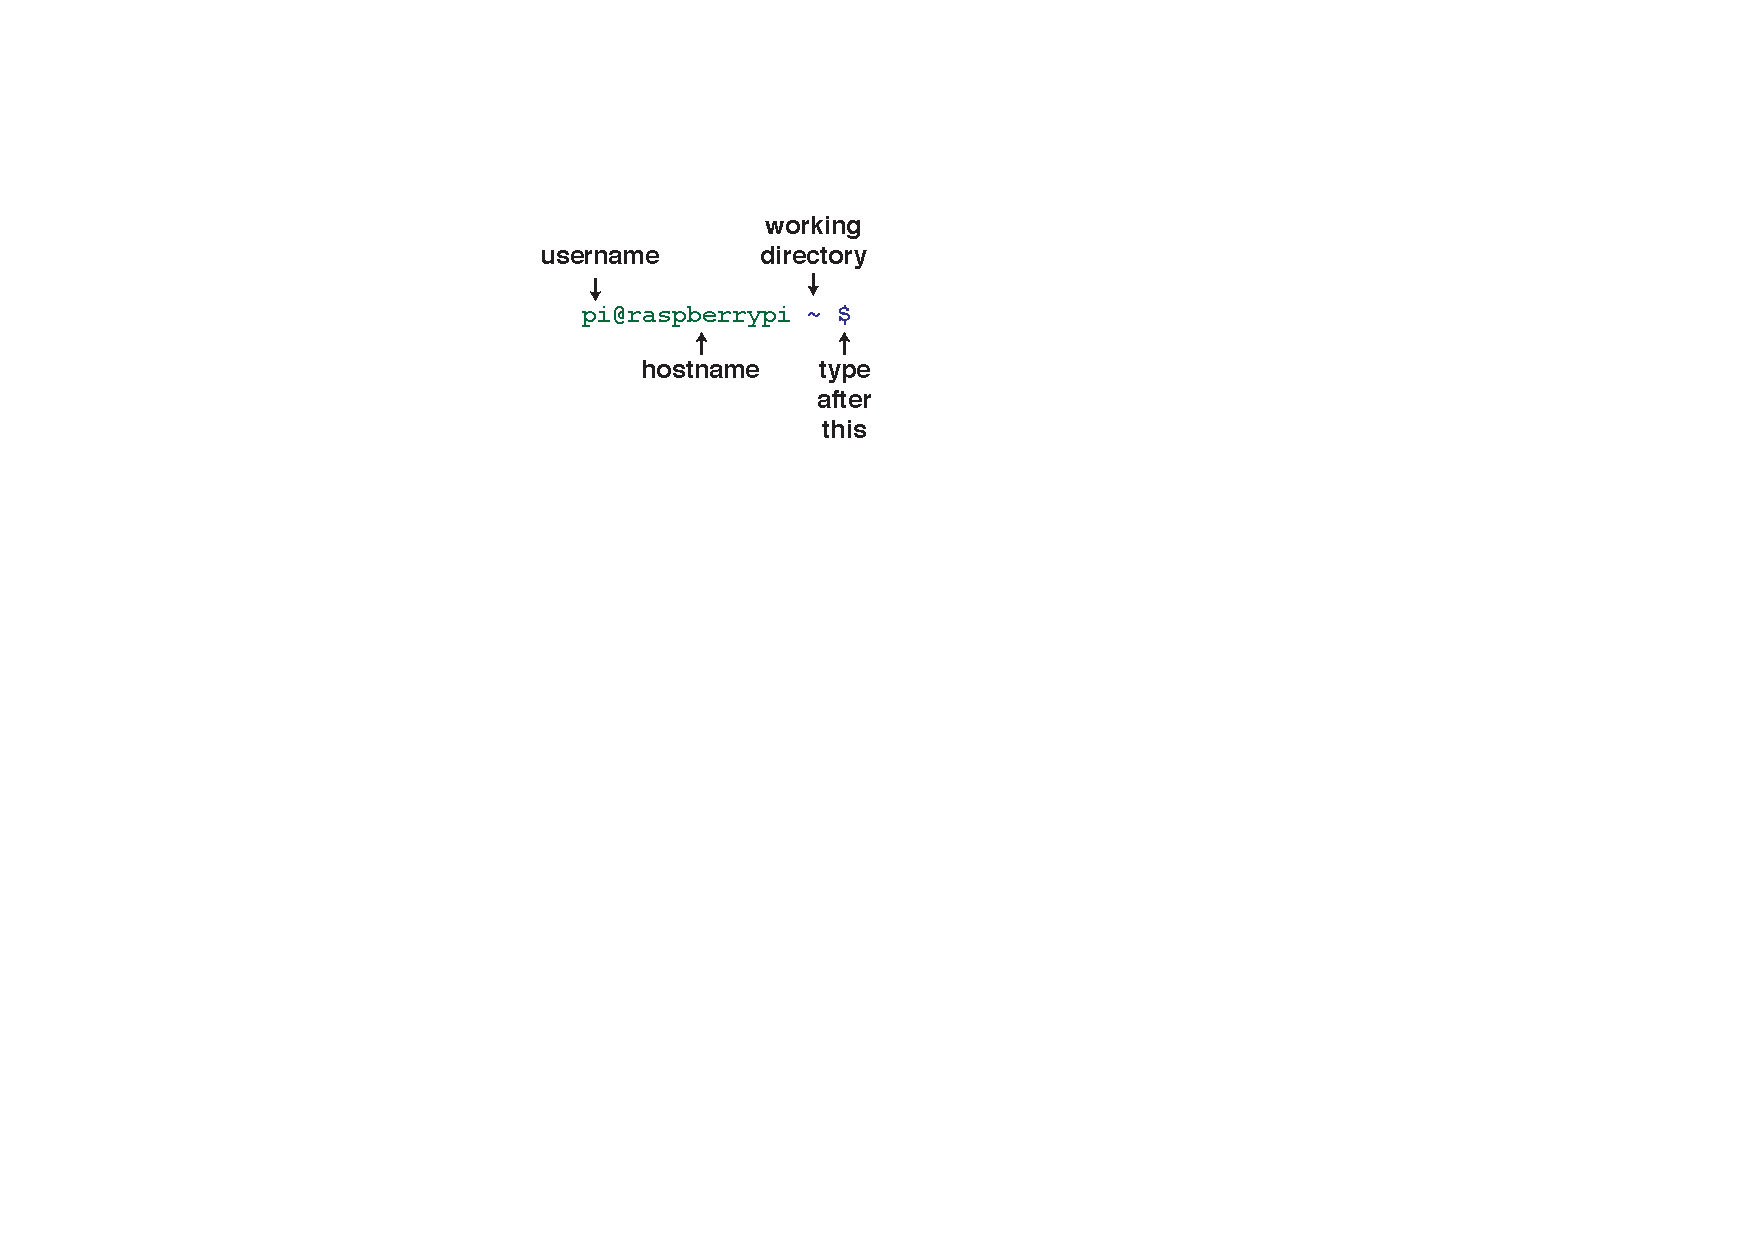
\includegraphics[width=7cm]{images/default-prompt}}
\caption{The different components of the Pi's default command prompt.}\label{figure:prompt}
\end{figure}


\begin{itemize}
\item To the left of the \ttout{@} symbol is the name of the user, and in this case that's \ttout{pi}, since you've just logged in under that name
\item To the right of the \ttout{@} is the hostname of the machine, which on a Raspberry Pi is quite reasonably set to \ttout{raspberrypi} by default.
\item The \texttildelow{} tells you where in the filestore you're currently working. We'll explain this in a lot more detail later on, for now all you need to know is that the \texttildelow{} symbol is called a \textit{tilde} (pronounced something like till-duh, though locally its often referred to colloquially just as a `twiddle'), and is used here to refer to the `home' of the current user. 
\item the \$ symbol signifies that you can type your commands from here on. 
\end{itemize}

You can change this prompt to something more or less verbose later, but for now we'll leave it as it is. For simplicity in these notes, we'll use the \$ notation from now on to mean `type something at the command prompt and press Enter'. So for example

\begin{ttoutenv}
$ echo Hello World
\end{ttoutenv}

\noindent means `type \totype{echo Hello World} at the command prompt and then press Enter' (you can do this if you like; the result will be that `Hello World' gets `echoed' back to you on the next line of the screen). 

Before we do any real work on the Pi, we should make it a bit more secure than it currently is. Remember, you've logged in using the default username `pi' and the default password `raspberry', so anybody else could do the same. To change the password to something that's unique. For inspiration and advice on creating good passwords, see Figure \ref{figure:xkcd-password}.

\begin{figure}
\centerline{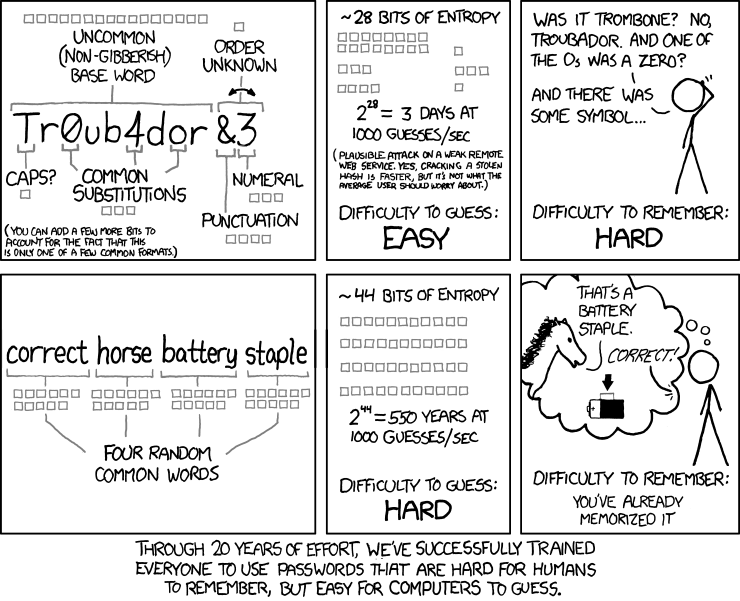
\includegraphics[width=13.5cm]{images/xkcd-password-strength}}
\caption{XKCD's take on password creation \url{http://xkcd.com/936/}}\label{figure:xkcd-password}
\end{figure}

The command to change the password is \totype{passwd}; typing this at the command prompt and entering your current (i.e. `raspberry') and new password (twice, to be sure), should look like this:

\begin{ttoutenv}
$ passwd
Changing password for pi.
(current) UNIX password:
Enter new UNIX password:
Retype new UNIX password:
\end{ttoutenv}

\noindent Note in the above, we're using lines that don't start with the dollar symbol to show output as a result of what you've typed, and that none of the passwords you're typing actually appear on screen for obvious sneaky over-the-shoulder-peeking reasons. \textbf{Don't forget this password: there's no easy way to get back into your Pi without resetting everything.}

\begin{danger}{Memory Loss} 
Although the Pi uses a fairly standard UNIX operating system, it's probably not quite as secure as a normal desktop machine because of its small size and easily-removable storage media. Once the Pi has booted from the SD card, it's about as secure as any other Linux machine. But because the memory card is easily removable, it can trivially be connected to another machine as a `removable media' device; and at that point the host machine can almost certainly see its contents, including any of the files you've created, because the filesystem itself isn't encrypted. And because the Pi is small and portable, it's easier to lose it than a laptop or desktop machine; so, be careful!
\end{danger}

Now that your password isn't the same as the `out of the box' Pi one, it's safe to plug your Pi into the network. There's a spare ethernet cable poking out of the desk; plug that into the appropriate socket on your Pi (number \circled{8} on Figure~\ref{figure:bare-rpi}) and you should see the FDX, LNK and 10M LEDs light up. To confirm that you're now connected to the network, use the \totype{ping} command, which sends a low-level network message to a designated place and checks for a response, to see if you can reach our School's web server. 

\begin{ttoutenv} 
$ ping www.cs.manchester.ac.uk
PING waldorf.cs.manchester.ac.uk (130.88.194.191): 56 data bytes
64 bytes from 130.88.194.191: icmp_seq=0 ttl=52 time=37.914 ms
64 bytes from 130.88.194.191: icmp_seq=1 ttl=52 time=40.392 ms
64 bytes from 130.88.194.191: icmp_seq=2 ttl=52 time=41.006 ms
\end{ttoutenv}

Each of the lines starting with `\ttout{64 bytes}' represents a short response from the machine you've just pinged, and you're shown the round-trip time for ping's data to leave your Pi, find (in this case) \fname{www.cs.manchester.ac.uk} on the network, and return back to your Pi. Since we're just using ping here to give us some confidence that the network is okay, we don't need to leave it pinging away for ages, so let's stop the ping command in its tracks. Hold down the control key (marked `ctrl' on the keyboard), and press `c'. This will signal the currently executing command that it should stop what its doing and return to the command prompt (quite often this is referred to as ``control-c'ing'' a command, and it will have the same effect on the majority of command-line tools).

\begin{diversion}{Ping}
  The \totype{ping} command is named after its use in the field of active sonar, where an actual `ping' sound was sent through water, and distance calculated by listening for the echo to return. It's the classic boingy pingy noise associated with submarine movies! 
\end{diversion}

\section{The Unix Shell}

Before doing anything else, let's take a step back and look in a bit more detail at what you've just done. You have been
interacting with a \wikipedia{Shell_(computing)}{shell}: a program that prompts
the user for commands, accepts them, executes them and displays the
results. A shell is just a program running on the Linux operating system like any other program---it's not `built in' to the operating system in any special way, it just happens that by default, the Pi is set up so that when a user logs in, the first program that gets executed on behalf of that user is an interactive shell that allows the user to execute further programs themselves. Later in this course we'll look at the file that determines which program gets executed first for a user, and indeed at the order in which programs are run by the operating system as it boots up, because in Linux all of these things can be easily configured by changing a few lines in the appropriate text file. But for now, it's enough to understand that the shell is just a program that interacts with the user via the keyboard and display, and allows you to execute commands to do useful things.

\begin{diversion}
Unix has many shells: the first shell was called the `Thompson' shell (also known as just `sh', and pronounced ``shell''), written by Ken Thompson for the first Unix system; then came the `Bourne' shell (also called `sh'), written for a later commercial version of Unix by Stephen Bourne. You have just been using the Free Software Foundation's `Bourne Again' shell (another pun-name taking a dig at its commercial fore-runner), or `bash'. The various different shells offer the user different facilities: `sh' is rather
primitive compared to the more modern ones. However, their basic
functionality is always the same: they accept commands from the
\textbf{standard input} (for now, we can treat that as meaning `the keyboard'), execute them, and display
the results on the \textbf{standard output} (i.e. for now `the screen', which in
this case was the entire screen, or \textbf{console}). Shells repeat
this process until they have reached the end of their input, and then
they die. Unix shells are rather like \textbf{Command Prompt} windows in Microsoft
Windows, except that Unix shells are considerably more sophisticated.
\end{diversion}

\section{The Unix File System}

Next we're going to explore the Pi's filesystem a little. You'll be familiar with the idea of a hierarchy of files and folders from whatever graphical environment you're used to using on desktop or mobile devices: files represents things that you've created or downloaded such as documents, images or movies, and folders are a way of organising these into related collections. By putting folders inside folders, you can organise your stuff starting with general concepts such as `Photographs' and ending up with much more specific collections, e.g. `Holidays', then `Bognor Regis 2013'. 

Interacting with a standard UNIX filesystem via the command-line uses similar concepts (actually, it's the graphical environment that's being `similar' here really, since the UNIX command-line existed quite some time before anything graphical appeared). Files are called files, but what are commonly represented as `folders' in graphical environments are more correctly called `directories' when we are operating at this level (and we'll call them directories from now on, because it'll make many of the command names make more sense). 

Let's first see what stuff we already have on our Pi. The \totype{ls} command lists files and directories. Type it now, and you should see that two folders have already been created for you, one called \fname{python\_games} and the other called \fname{Desktop}. 

\begin{ttoutenv}
$ ls
Desktop python_games
\end{ttoutenv}

When we're using a command-line prompt, we have the notion of of \wikipedia{http://en.wikipedia.org/wiki/Working_directory}{current working directory} which is the directory that we're currently `in'. Any commands we issue that don't specify another directory are assumed to refer to the current working directory; so \totype{ls} on its own really meant `run the list command on my current working directory'. 

Let's say we want to look at the contents of the \fname{python\_games} directory. There are several ways of doing this, but for now we'll break the process down into simple steps. Use the \totype{cd} command to Change Directory to \fname{python\_games}:

\begin{ttoutenv}
$ cd python_games
\end{ttoutenv}

\noindent and then use the \totype{ls} command to list its contents. You should see a long list of files: some are programs written in the Python programming language (these files end in .py), others are images or sounds used by those programs (ending in .png or .wav). At the prompt type:

\begin{ttoutenv}
$ python wormy.py
\end{ttoutenv}

to start a simple version of the classic `Snake' game. You can guide your green snake around the screen with the cursor keys; you score a point every time you eat one of the red squares, and extra segment gets added to your snake. The game finishes if you crash into the edge of the screen or eat yourself. Once you've convinced yourself this is working (don't spend too long playing the game!), press the Escape key to return to the command prompt. You'll be writing a more sophisticated version of this game soon enough in the Java labs.

Take a look now at the command prompt; whereas before it was just
\\
\\
\totype{pi@raspberrypi \texttildelow{} \$}
\\
\\
it has now become
\\
\\
\totype{pi@raspberrypi \texttildelow{}/python\_games \$}
\\
\\
to indicate that we've changed our current directory to \fname{python\_games} (remember the \texttildelow{} symbol means `home directory', so \fname{\texttildelow{}/python\_games} really means 'a subdirectory called python\_games which is in my home directory').

%\FloatBarrier
\section{The UNIX filesystem}

In UNIX, as with most other operating systems, the files and directories you create can have more-or-less any name you like. It is very sensible to give them names which mean something and make their purpose clear. This is despite some of the traditional file names in Unix being rather cryptic---this is particularly true for most UNIX commands. You'll get used to that. 

\begin{danger}{File name formats}
The filesystem on your Pi (which uses a type of filesystem called `ext4') \textit{case sensitive}, which means that \fname{Hello.txt} and \fname{hello.txt} are treated as different files because they have different case letters in their names. The filesystem used by Microsoft Windows since XP (called `NTFS') is also case-sensitive. Apple's OS X, however uses `HFS Plus' (which usually appears as `Mac OS Extended (Journaled)'), and this is not a proper case-sensitive file system; although it will remember whether you called a file \fname{Hello.txt} or \fname{hello.txt} so files \textit{appear} to be case sensitive, the OS itself treats them as being \textit{the same file}! The same is true for the FAT32 filesystem used on most removable USB drives -- because it's one of the few formats that's understood by Windows, Mac and Linux. 

Most of the time this isn't a problem, but you should be careful of the effects when copying files from one filesystem to another, especially if you are using a USB drive to transfer files from a Linux box to somewhere else. For example, if you have two files in the same directory on Linux but with different capitalisation, one file will overwrite the other when you copy them onto your USB drive (and which one survives will depend on the order in which they are copied). One way around this problem is to use something like \totype{tar} or \totype{zip} to bundle the files up into a single archive file, and then transfer that via the USB drive. 
\end{danger}

\begin{linux}{Spaced out filenames}
Because of its roots in the early days of computing long before the advent of graphical user interfaces, UNIX filenames tend not to have spaces in them because this conflicts with the use of a space to separate out commands and their parameters. The UNIX filesystem does allow spaces in filenames, but you'll have to use a technique called `escaping' if you want to manipulate them from the command line; this involves prefixing spaces in filenames with the backslash character \textbackslash{} to tell the command line not to interpret what follows the space as a new parameter. For example, a file called \fname{my diary.txt} would be typed as \fname{my\textbackslash{} diary.txt}. It's a bit ugly, but it works fine. 
\end{linux} 

As you already know, directories are created within directories to create a hierarchical structure. But where is the `top' directory? Surely that has to go somewhere? On each machine, there is one directory called `/' which is referred to as the \textit{root}, which is not contained in any other directory. All other files and directories are contained in root, either directly or indirectly. The root directory is written just as \fname{/} (note this is the opposite slanting slash character to that used in Windows, which means something similar but different). 

If we wish to talk about the file \fname{y} within the directory, \fname{x} we write \fname{x/y}. Of course, \fname{y} may itself be a directory, and may contain the file \fname{z}, which we can describe as \fname{x/y/z}.

You can think of this structure as defining a tree, with \fname{/} as the root (hence its name), directories as branches, and other files as leaves. You will study trees as abstract data structures, later in this year, and in Year 2, but this simplified model of the Unix file system structure will do for now. 

One really important, and slightly strange thing to get used to, though, is that computer science trees grow upside down, so although we call them trees, the `root' is usually thought of as being at the top, and the `leaves' at the bottom. You'll hear phrases like `go up to the root directory, and then down one level to the home directory'. We normally think of the root directory as being at the top of the tree. (For those of you who are interested: Unix actually allows links, which means the structure can really be a cyclic graph. Links are similar to, but fundamentally not the same thing as, shortcuts in Windows.)

Apart from \fname{/} there are two more directories of special note:
\begin{itemize}
\item Your \textit{home directory} is the directory where you find yourself when you log in. It might be tempting to think of this as being the `top' of the tree (and for every-day purposes thinking this way is probably okay), but in reality your home directory is probably one or more levels away from the root of the file system. We'll find out where this is on the Pi shortly. 
\item Your \textit{current working directory} is the one you are working in at a particular moment. \end{itemize}

So let's see where we are in the Pi's filesystem at the moment. Assuming you're following these instructions properly you should still be in the \fname{python\_games} directory (check the command prompt to confirm this is the case). To go back to our home directory, we can use the \totype{cd} command without any parameters:
\begin{ttoutenv}
$ cd
\end{ttoutenv}

You should see the command prompt change back to being as it was when we first logged in. So where in the filesystem is our home directory? We can find out where we currently are using the \totype{pwd} command, which stands for Print Working Directory:

\begin{ttoutenv}
$ pwd
/home/pi
\end{ttoutenv}

So apparently we're in a directory called \fname{/home/pi} which sounds plausible enough. Notice that the \totype{pwd} command has returned us an \textit{absolute pathname}, because \fname{/home/pi} starts with a \fname{/} character, so we now know that the home directory for the user \fname{pi} is in a directory called \fname{home} which itself is a subdirectory of root. 

Let's confirm that this is true. Issue the command:
\begin{ttoutenv}
$ cd /
\end{ttoutenv}

which just means `change directory to the root directory' and use the \totype{ls} command to look at the root directory's contents. You'll see several directories with names like \fname{bin}, \fname{boot}, \fname{dev} and \fname{lib}. Most of these contain `housekeeping' files for the operating system, and at this stage you don't need to know what's in them (though Table \ref{table-dirs} gives you a brief description if you're interested). The one called \fname{bin} is quite interesting though, so let's investigate that by typing: 

\begin{ttoutenv}
$ cd bin
$ ls
\end{ttoutenv}

\noindent You should see a fairly long list of files. Look carefully, and you'll find two names that you recognise: \totype{ls} and \totype{pwd}. These are the `binary executable' files for the commands that you've just been using (which is why they are in the `bin' directory, which is short for binary). In UNIX, most commands are not `built into the system', but are just programs put in a special place in the filesystem that are picked up by the command-line when you type things. This makes UNIX very easy to extend with new features; you just write a program to do what you want, and put it in the right place. We'll look at how the system knows where to find commands later, and explore several of the other commands you can see in this directory as well. 

We now need to get back to our home directory. You should by now be able to think of at least four different ways of getting there!

\begin{enumerate}
\item \totype{cd} on its own means `take me directly to my home directory'.
\item We know that the tilde symbol also means `my home directory', so \totype{cd \texttildelow{}} will also work (though at the expense of two extra keystrokes!)
\item We could go back to the root directory by first typing \totype{cd /}, then \totype{cd home} and finally \totype{cd pi}, or 
\item We could go straight from where we are now (which in \fname{/bin}, remember) by typing \totype{cd /home/pi}. 
\end{enumerate}

Now we're back in our home directory (check the command prompt to make sure), you may have noticed that our commands for navigating around the filesystem are missing one feature. We can go to the `top' of our home directory easily enough; and we can go straight to very top of the whole filestore using \totype{cd /}; and we know how to descend into a subdirectory (e.g. \totype{cd python\_games}). But how do we go up one level? If we were in some nested subdirectory several levels below our home, and wanted to go just one level back up the tree, it would be very tedious to have to start back at our home directory and traverse back down to where we wanted to be. 

UNIX represents the idea of going `up' one directory with the \fname{..} symbol (that's two fullstops typed immediately after one another with no spaces). So if you are in, say, \fname{python\_games} and want to go \textit{back up} to the directory above, you could type:

\begin{ttoutenv}
$ cd ..
\end{ttoutenv}

You can mix in the \fname{..} notation in relative and absolute paths anywhere you like. So, assuming you are still in \fname{python\_games}, how could you get into \fname{/bin} using only a \textit{relative} path in the \totype{cd} command? Yes, this is a slightly artificial exercise because the simplest solution would just be to use the absolute path \totype{cd /bin}, but just go with the flow for now and work it out using a relative path. The answer is shown in Figure \ref{figure:simple-navigation}. 

\begin{figure}[t]
\centerline{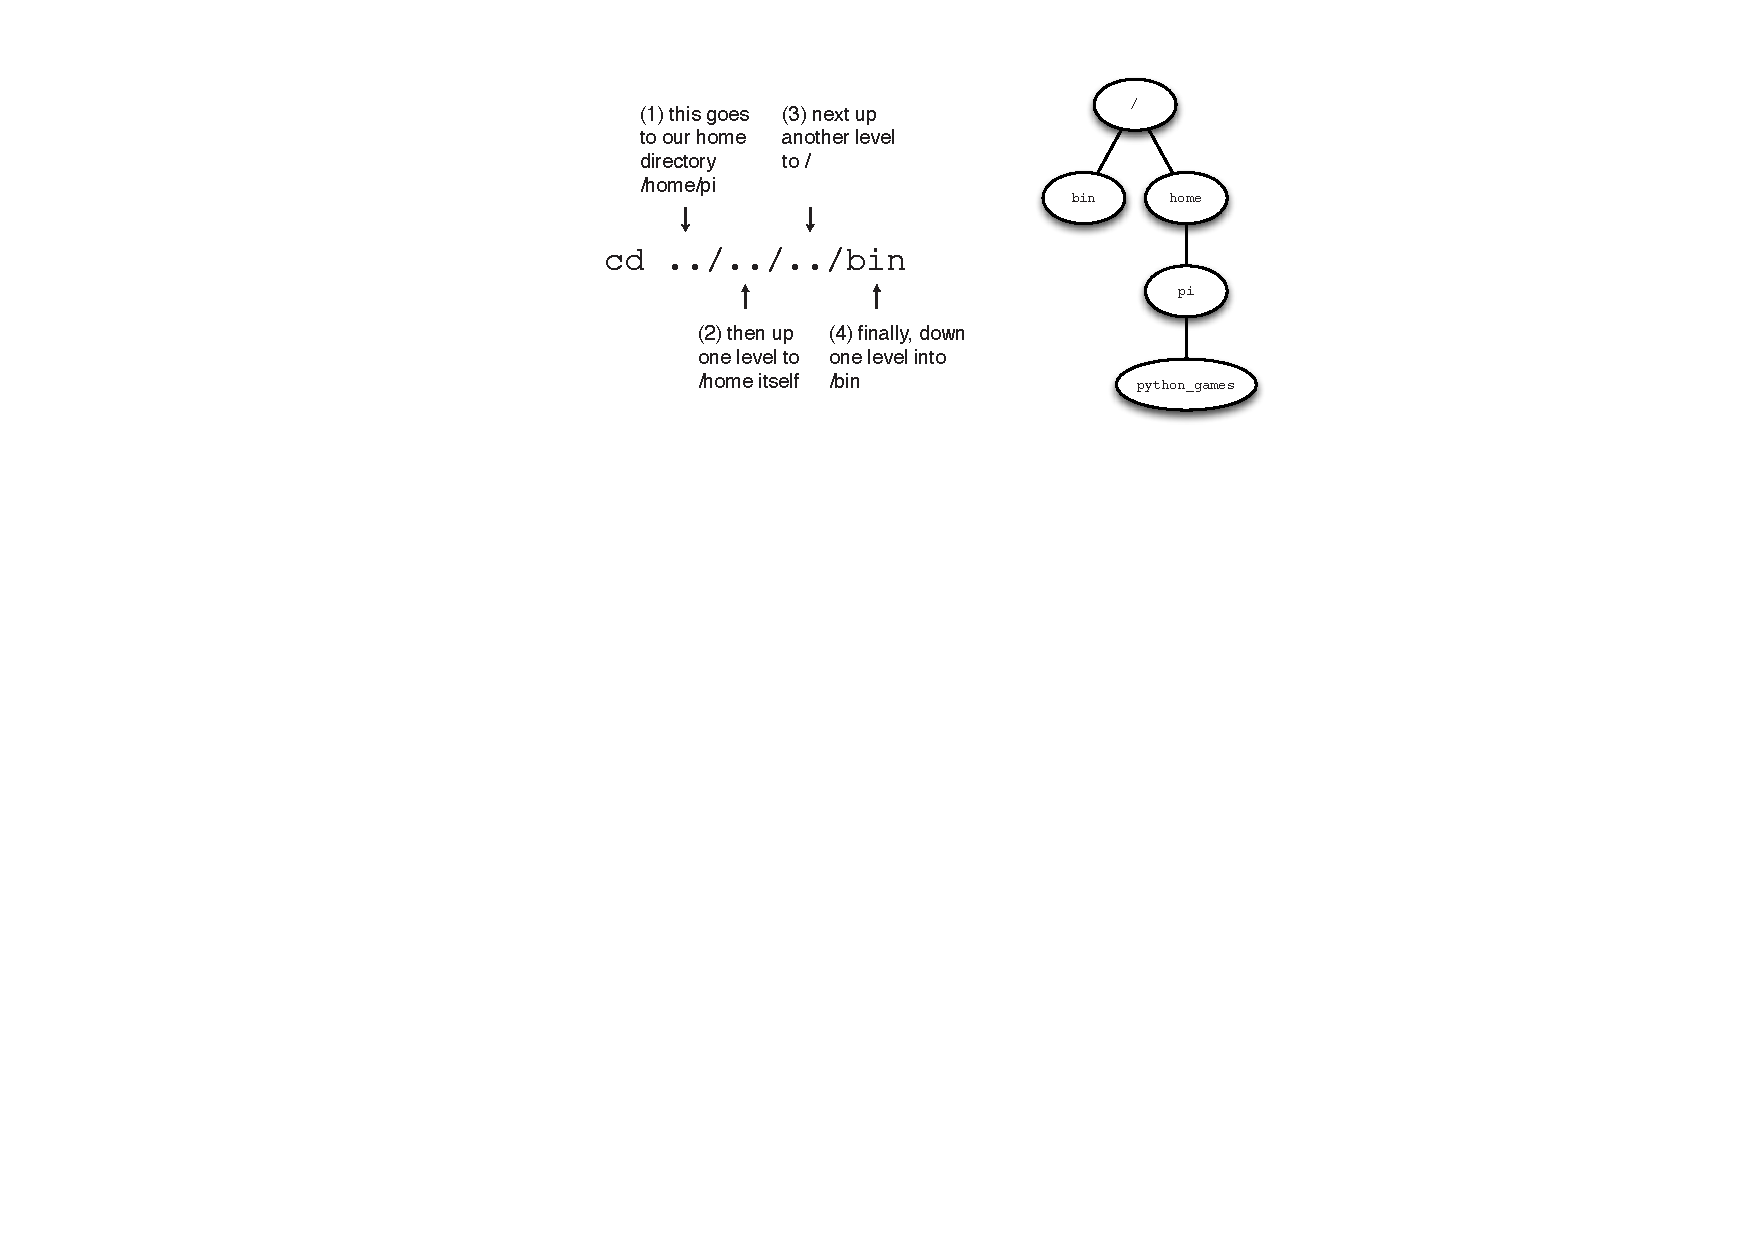
\includegraphics[width=13.5cm]{images/simple-navigation}}
\caption{Given the Pi's default filesystem structure, starting in the \fname{python\_games} directory, the command \fname{cd ../../../bin} will take you to the \fname{/bin} directory (by an admittedly tortuous route!)}\label{figure:simple-navigation}
\end{figure}

%\FloatBarrier
\section{The Colossal Cave}

We're now going to explore a bit of computing history, and install and play one of the very early computer games. Colossal Cave Adventure was the first `adventure game', in which a virtual world is described using only text, and the player controls the game's protagonist using simple textual commands. The game was created in 1976 by a keen caver called \wikipedia{William_Crowther}{Will Crowther} who at time was a programmer at Bold, Berenek \& Newman, the company that developed \wikipedia{ARPANET}{ARPANET}, the forerunner to the modern Internet. He later collaborated with \wikipedia{Don_Woods_(programmer)}{Don Woods}, then a graduate student at Stanford University, to create the Colossal Cave Adventure as we would recognise it today. The original version consisted of around 700 lines of \wikipedia{Fortran}{FORTRAN} code and a similar number of lines of data. When running on a \wikipedia{PDP-10}{PDP-10} (see Figure~\ref{figure:cern-pdp-10} for a picture of what one of these machines looked like) would consume around half of the machine's memory. To put this in perspective, the tiny Raspberry Pi computer on your desk has roughly 1000 times as much memory as the PDP-10; it can run Colossal Cave with ease. 

\begin{figure}[t]
\centerline{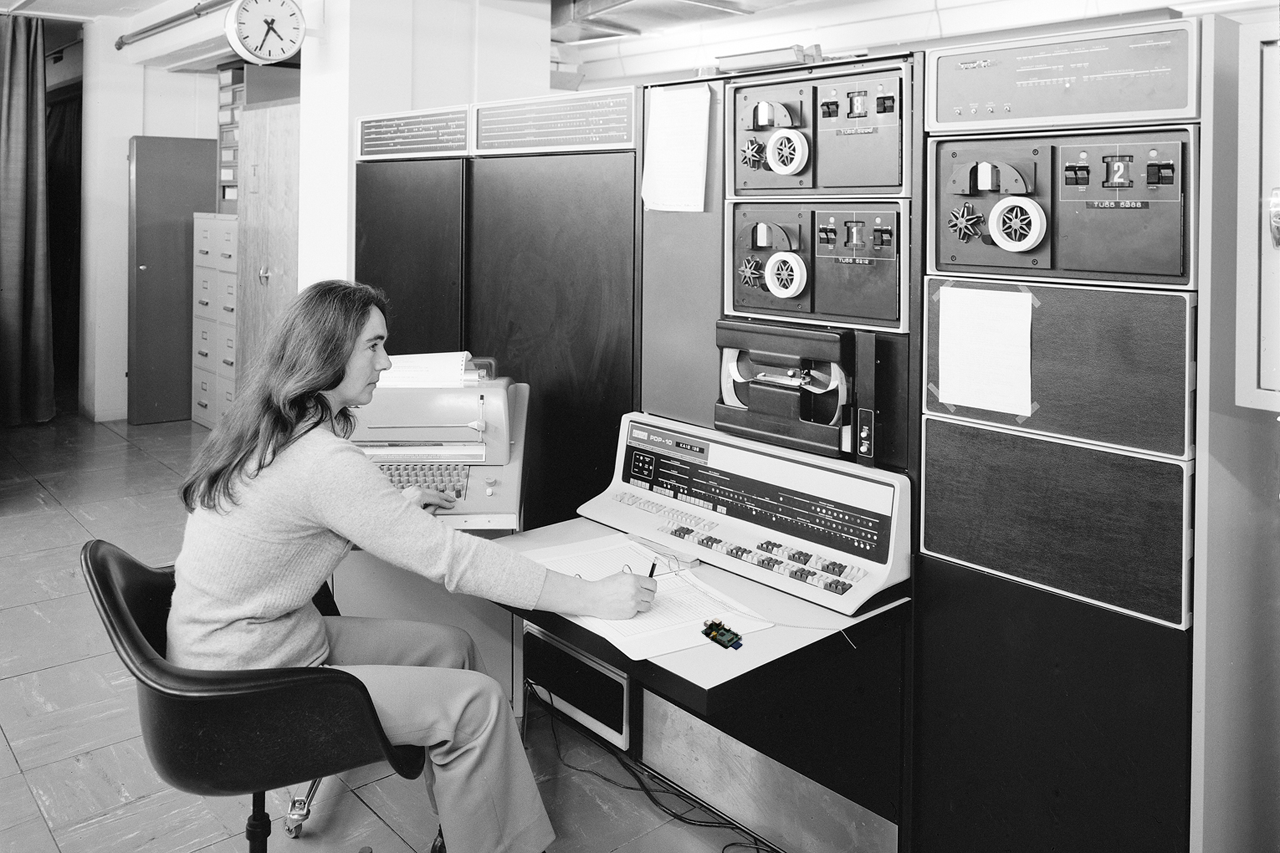
\includegraphics[width=14cm]{images/cern-pdp10+pi.png}}
\caption{A PDP-10 from CERN, circa 1974, reproduced with permission. \url{http://cds.cern.ch/record/916840}. We've taken the liberty of crudely superimposing a Raspberry Pi to approximately the right scale on the operator's desk, just to give a sense of the difference in size between the two machines.}\label{figure:cern-pdp-10}
\end{figure}

Although the original FORTRAN source code for Colossal Cave still exists, the version you're going to play with is based on a re-implementation of the game on what became known as the \wikipedia{Z-machine}{Z-Machine}: a virtual machine specifically for running interactive fiction games.\footnote{Don't confuse the Z-machine, which is a virtual machine for adventure games, with the Z Machine, which is the largest X-ray generator in the world. Doing so is likely to make your lamp melt, and the trolls very grumpy.}
 
\FloatBarrier
\section{Installing Frotz, a Z-Machine Interpreter}

Unlike the other commands that you've used so far, the program we need to be able to play Colossal Cave Adventure isn't pre-installed on the Raspberry Pi, so we're going to have to fetch and install it ourselves. Fortunately, the version of Linux that we have on the Pi comes with a package management system that makes this quite easy. 

But first, we're going to have to understand a command called \totype{sudo}. Everything that you've done so far has involved looking at files that either belong to the `pi' user, or are parts of the system that can be read or executed by any user. But of course, installing a new piece of software involves not just reading, but \textit{modifying} the Pi's operating system in some way, and that's not something that you want to do casually since mistakes could potentially mess up whole device. 

You'll be familiar with the idea of a user with Administrator privileges from Windows or OS X; on Linux the `superuser' that can do anything to any part of the system is called `root' (because this user can modify any part of the system from the root of the filestore downwards). In the early days of UNIX, administrators would log in as the root user to modify, update and repair the system. This had two major downsides: first, that if you accidentally left yourself logged in as the superuser when you nipped out for a coffee, the machine was vulnerable to misuse by anybody who would get at the keyboard; but second and more serious, all the normal safety nets that prevent you from accidentally deleting or damaging the operating system itself are deactivated, so its much easier for a slip of the finger or a brief moment of stupidity to have disasterous effects. To avoid these problems, UNIX systems now usually recommend the use of the \totype{sudo} ('Super User Do') command to temporarily elevate a normal users' privilege that that of super user for a single command. 

The system that we're going to use to install this game is called \totype{apt}, which stands for Advanced Packaging Tool. The \totype{apt} maintains a list of remote \textit{repositories} in which packages have been put that contain all the executables, libraries and data files necessary to install a particular Linux program. It can deal with fetching packages over the Internet, as well as extracting and copying their contents into the right places on your system. It also performs a series of sanity-checks to make sure that what you're adding is compatible what whatever you've already got in place.

The system we want to install to play this game is called \textit{frotz} (to learn why, you'll have to play the game a bit!) Let's try running the \totype{apt-get} command \textit{without} having gained superuser privilege first. Try typing:

\begin{ttoutenv}
$ apt-get install frotz
\end{ttoutenv}

\noindent The operating system will respond with something like:

\begin{alltt}
  \small
E: Could not open lock file /var/lib/dpkg/lock - open (13: Permission denied)
E: Unable to lock the administration directory (/var/lib/dpkg/), are you root?
\end{alltt}

Notice the question at the end: `are you root?'. Well, no you're not, so Linux has rightly prevented you from performing this operation. Now we'll try again using the \totype{sudo} command. This time type:

\begin{ttoutenv}
$ sudo apt-get install frotz
\end{ttoutenv}

You should see a series of lines printed out on the console, ending with:

\begin{ttoutenv}
Setting up frotz (2.43-4) ...
\end{ttoutenv}

\noindent before being returned to the command prompt (note the version number for frotz may have changed from 2.43-4 by the time you use this tutorial, don't worry, that's fine). It's possible that \totype{apt-get} will fail to find the frotz package in one of the repositories it knows about; if this happens, it's usually because the repository has moved somewhere else on the internet, so you need to tell the APT system to update itself first: run the command \totype{sudo apt-get update}, and when that has completed try installing the frotz package again, and all should be well. 

\begin{rpi}{APT}
The APT system is a very convenient way of managing packages, since it will automate the process of finding, fetching, configuring and installing software on your Pi (or indeed, on other Debian-based Linux installations). The RPM system does something similar for distributions based on Red Hat's version of Linux.

The various repositories that contain the packages for your Pi are updated regularly, so it's worth running \totype{apt-get update} once in a while to refresh your Pi's list of software. 

You should also at some point run \totype{apt-get upgrade}, which will cause all the packages that have already been installed to be upgraded to the latest version that the APT system can find. This lab will work just fine with the versions of software that are pre-installed on your Pi, and the upgrade process can take quite some time (hours, possibly), so you mustn't do it now or you won't be able to complete this lab in time. Try it at home, or outside of a lab session. 
\end{rpi}

The frotz system on its own is just a virtual machine into which you can load adventure game data, so we'll need to fetch the Colossal Cave datafile before we can play anything. We've put a copy of the game at \url{http://pod.cs.man.ac.uk/COMP101/Advent.z5} so you can fetch it from there.

Oh, hang on. No web browser. Oh dear.

Although it is actually possible to browse the web in console mode on the Pi (we'll experiment with this in the next lab session), there's an easier way to interact with the web to get the file that we need, using a command called \totype{curl}. First, use \totype{cd} to change to your home directory if you're not there already, then

\begin{ttoutenv}
$ curl http://pod.cs.man.ac.uk/COMP101/Advent.z5 -o Advent.z5
\end{ttoutenv} 

\noindent and you'll see \totype{curl} fetch the file you need `over the web' and save it in your home directory. This is also the first time you've encountered what's called a command-line parameter \textit{switch}: the \ttout{-o} parameter tells \totype{curl} to use the next parameter it sees as the filename for the thing it's fetched from the URL given as its first parameter. More on switches later. 

Use \totype{ls} to confirm that you can see the file \fname{Advent.z5} in your home directory, then type: 

\begin{ttoutenv}
$ frotz Advent.z5
\end{ttoutenv}

\noindent to start playing the Colossal Cave Adventure. Once the game has started (the sceen will have gone blue), type HELP to get instructions. When you've had a bit of a wander around and got the general idea of the game, you can type quit to get back to the command prompt. There's a map of the entire Colossal Cave world at the back of this exercise.

Earlier, we referred to Colossal Cave as a work of Interactive Fiction (IF). In truth, this is perhaps stretching the term somewhat, since the genre has matured considerably in the decades since this first adventure game. For a much more compelling example of Interactive Fiction with beautifully written prose, and funny and challenging puzzles we suggest you have a go at playing Curses by \wikipedia{Graham_Nelson}{Graham Nelson}, or one of the many other games written by Interactive Fiction enthusiasts that are available for free from \url{www.ifarchive.org}. If you find yourself getting hooked on playing IF, the frotz interpreter is available for most platforms, including iOS, Android, OS X and Windows. 

We'll finish this lab session off with one more game. 

Use {\tt curl} to fetch the file hosted at \url{http://pod.cs.man.ac.uk/COMP101/quake3.tar.gz}, making sure you save it in your home directory. 

Notice that this file ends with \fname{.tar.gz}. The \fname{.gz} suffix tells us that this file has been compressed using a utility called \totype{gzip}, so the first task is to uncompress the file. Type:

\begin{ttoutenv}
$ gunzip quake3.tar.gz
\end{ttoutenv}

This will uncompress the file, removing the \fname{.gz} and leaving you with \fname{quake3.tar}. A `tar' file a bundle of individual files that have been assembled together into a single file for convenience. The name `tar' is an abbreviation of 'Tape Archive', since the \totype{tar} command was originally used for making backups of filestores onto tape. It remains, however, a very versatile way of bundling up lots of things, and you'll find tar files all over the internet. 

To see what's in this archive, run the command 

\begin{ttoutenv}
$ tar tf quake3.tar
\end{ttoutenv}

\noindent and you'll see a long list of the archive's contents scroll past on the screen. The first parameter to \totype{tar} is a bit of an odd one, since it's a collection of options, which unusually for UNIX are not prefixed by individual minus signs (recall the \ttout{-o} option we used for \totype{curl}; that's a far more common way of specifying options to tools). In this case the options mean:

\begin{itemize}
\item the \textbf{t} causes \totype{tar} to list the `table of contents', for the archive, without extracting anything.
\item the \textbf{f} tells tar that the next parameter is the file containing the archive. 
\end{itemize}

\noindent To actually extract the contents of the archive we issue the command:

\begin{ttoutenv}
$ tar xvf quake3.tar
\end{ttoutenv}

\noindent where

\begin{itemize}
\item \textbf{x} means `extract'.
\item \textbf{v} means `be verbose, and show what you're extracting as you do it'.
\item \textbf{f} again means `and here is the file to work on'.
\end{itemize}

\noindent When tar has finished working you're presented again with the command prompt. Use \totype{ls} to confirm that you now have a directory called \fname{quake3} in your home directory. Now disconnect the mouse from the desktop PC, and plug it into your Pi; like the keyboard, it's connected to an inline USB socket so you don't need to rummage around behind the computer---and again, please remember to re-attach it to the main PC when you're done here. You might also want to plug some headphones into the Pi at this point too, if you happen to have a pair with you. 

\begin{ttoutenv}
$ cd quake3
$ ./ioquake3.arm
\end{ttoutenv}

\noindent After the startup screen, the game will ask you for a code, but you can just skip this and use the mouse to select the play option. The rest, we're sure, you can figure out for yourself. 

\begin{diversion}{Multiplayer Quake?}
You can play this version of Quake3 Arena with friends over the network. We'll leave you to figure out how to configure that yourself (hint: the \totype{ifconfig} command will tell you what IP address has been allocated to your Pi).
\end{diversion}. 

\FloatBarrier
\section{RTFM}

Although we've introduced several UNIX commands in this lab, we've only done so quite superficially today, giving you just enough detail to get through the tasks in this tutorial. Each of the commands is much more powerful than what you've been exposed to so far. Though you won't need to know every possible option off by heart, there are a lot of useful things you can learn about them quite easily. 

Most UNIX systems, including the one on your Pi have an instruction-manual system that gives more details about the available commands (and most things that you install yourself, such as \totype{frotz} also install their own manual pages).  Try running:

\begin{ttoutenv}
$ man ls
\end{ttoutenv}

\noindent for information on the \totype{ls} command, and use the same trick to find out more about the other commands you've seen today. If you need more help on how to use the \totype{man} command, you can always use: 

\begin{ttoutenv}
$ man man
\end{ttoutenv}

\noindent When you're looking at a manual page, pressing the Space Bar will advance you on a page, and the Up and Down cursor keys will move you back and forth line-by-line.

\begin{diversion}{RTFM?}
The acronym RTFM stands for Read The Flipping Manual, and is sometimes used as a response when somebody has asked a lazy question on a forum or by email where decent documentation already exists and is easily accessible. The F is usually interpreted as meaning something less polite than `Flipping'. 
\end{diversion}

\FloatBarrier
\section{Shutting down your Pi safely}
\label{section:shutdown}

When you're finished playing Quake, exit the game and get back to the command prompt. Like any other computer, its really important that you shut your Pi down properly; if you just pull the power chord out there's a chance of corrupting the filesystem. To shut the Pi down safely, type:

\begin{ttoutenv}
$ sudo halt
\end{ttoutenv}

\noindent You'll see the a series of messages scroll past that look rather like those you saw during the boot process. This shouldn't be surprising, since what the operating system is doing now is shutting down all the things that it started up when you booted the machine, roughly in reverse order. When all these services have closed down tidily, the Pi will power itself down; the network
 and OK LEDs will go off, the screen should go black, and only the red PWD LED will remain lit on the circuit board. At this point its safe to pull the Micro-USB cable out of the Pi. 

\FloatBarrier
\section{What have you learned?}

It might seem like you've been playing games for most of the lab, but if you've followed the instructions carefully and read through all the text you'll have learned a lot of new things. These include:
\begin{itemize}
\item the anatomy of a pi
\item how to safely start and stop your Pi
\item running commands: tar, cd, ls, pwd, unzip, sudo
\item how the filestore is structured
\item basic apt commands
\end{itemize}

\begin{table}
\begin{tabular}{lp{12cm}}
\hline
Directory & Description\\
\hline
boot & Contains the Linux kernel and other low-level packages needed to get the Pi to boot.\\
& \\
bin & Contains the binary executables for basic commands such as \totype{ls} and \totype{pwd}.\\
& \\
dev & This is a virtual directory that represents devices connected to the Pi as though they were files that you can read from and write to. \\
 & \\
etc & Contains configuration files used by various programs, and also the names and encrypted passwords of users\\
 & \\
home & Each user gets their own subdirectory of \fname{home}. \\
 &\\
lib & This is where \textit{libraries} are stored; these are bits of code that are shared between several programs.\\
 & \\
lost+found & If something bad happens and the system crashes half way through doing something, it will put a copy of files that it knows are in a broken state here.\\
media & When you mount removable storage devices such as USB memory stickets, they will appear as filesystems here.\\
 & \\
mnt & This directory is used to mount storage devices. \\
& \\
opt & When you install optional software that's not considered part of the operating system, it usually ends up here.\\
& \\
proc & Like dev, this is a virtual directory. This one contains accounting information about the various processes that are running on your Pi.\\
& \\
selinux & Contains utility files relating to Security Enhance Linux.\\
& \\
sbin & This contains special executable binary files associated with system maintenance.\\
& \\
sys & Various files needed by the operating system.\\
& \\
tmp & Many programs need to create temporary files as part of their execution; they go here, and get deleted when the system reboots.\\
& \\
usr & User-accessible programs and bits of configuration.\\
& \\
var & Another virtual directory, used by programs to store variables.\\
\hline
\end{tabular}
\caption{Standard Linux system directories.}\label{table-dirs}
\end{table}

\clearpage
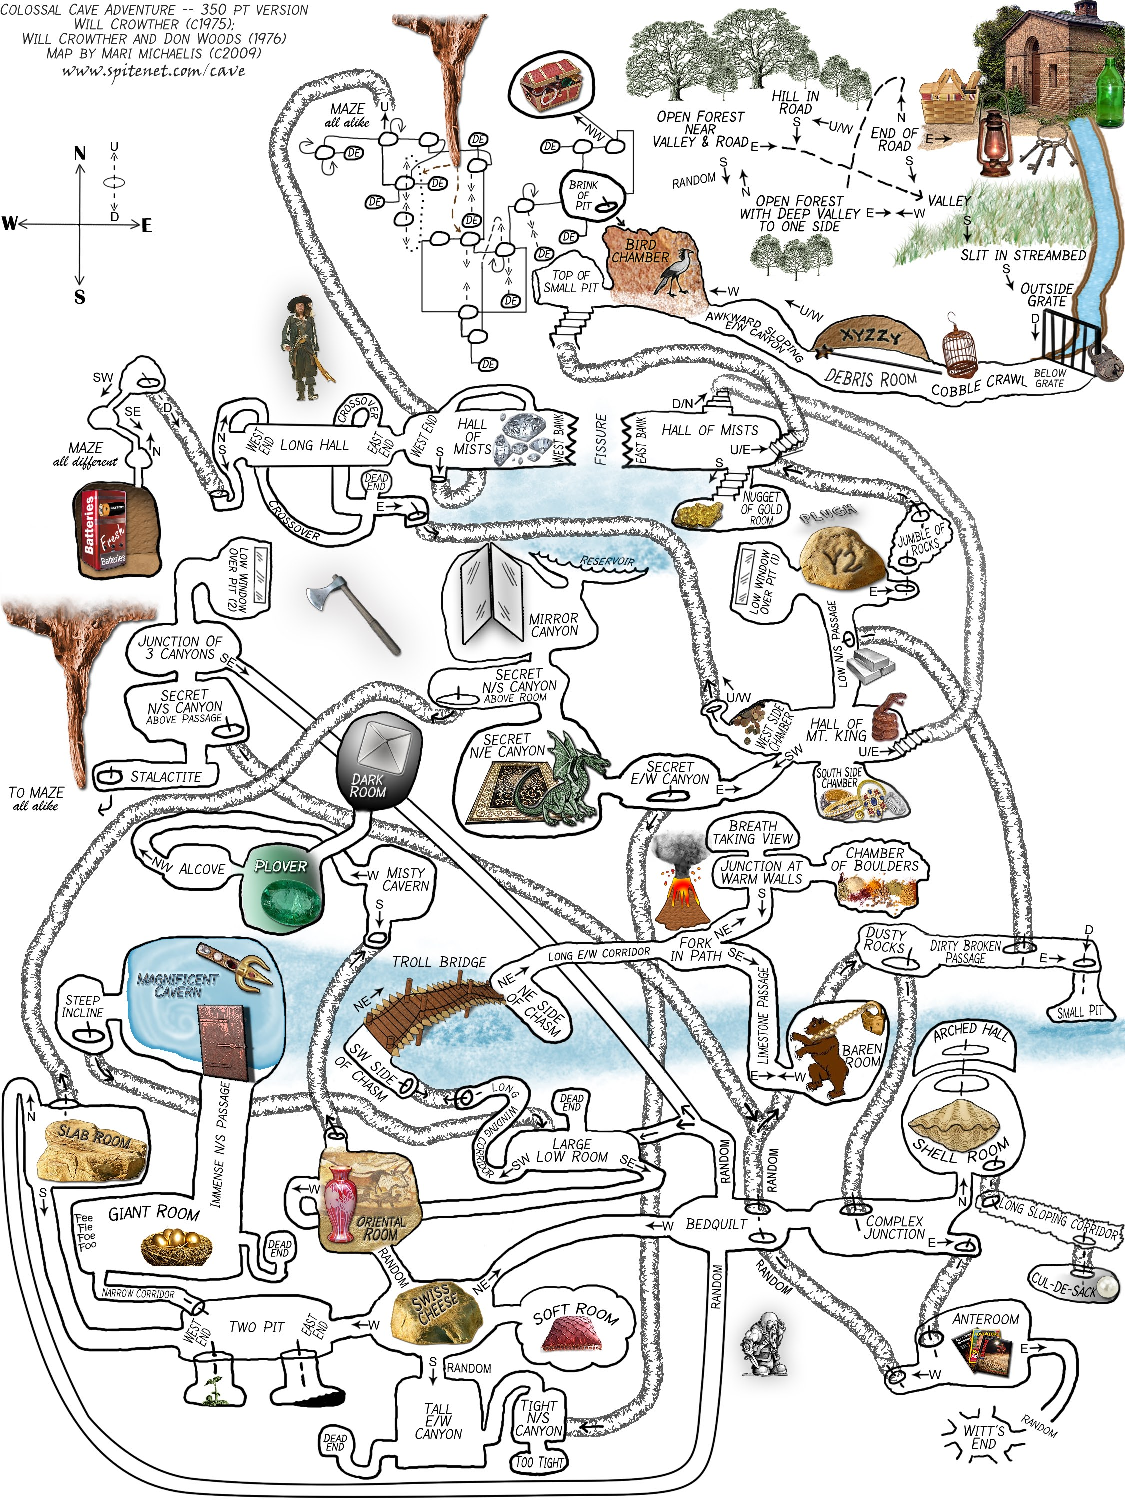
\includegraphics[width=15cm]{images/ColossalCaveAdventureMap}\\
\\
This map of Colossal Cave is reproduced here by kind permission of its author, Mari Michaelis. This is the `spoilers' version of the map, and contains clues as to how to solve the various puzzles in the game. If you want to play the game for real, you probably should make your own map, or at least use the spoiler-free version of the map available at \url{www.spitenet.com/cave}.

%\printbibliography


\chapter{Pi power}
\minitoc
\notesurl{rpi2}

So far you've used your Pi and the lab PCs separately, and hopefully you've come to understand that they are both essentially the same kind of machine; they both run variations of the same operating system, and the principles you learn using one for the most part apply to the other. In the case of the Pi, you have complete control of the device as a superuser, so can do absolutely what you like to it; in the case of the lab machines you have access to much more powerful hardware, but more restricted access to the filestore and operating system for reasons of security and privacy. 

Today, we'll be getting your Pi and a desktop PC to communicate with one another, to reinforce the similarities between these setups, and to expose you to some of the principles of networking and remote access. 

\section{The LXDE window manager}

Connect your Pi up to the monitor, keyboard, mouse, network and power supply as before, and log in (remembering this time to use whatever password you set on the Pi rather than your University password, and the username `pi'). At the console, type:

\begin{ttoutenv}
$ startx
\end{ttoutenv}

to start up X Windows and the Pi's default window manager, LXDE, which appear moments later looking like the screenshot in Figure \ref{figure:lxde-desktop}. 

LXDE (the `Lightweight X11 Desktop Environment') is designed to be a lean, fast desktop environment, which makes it ideally suited for the Pi's modest CPU. Although rather less rich in features and `eyecandy' than Gnome, LXDE is a fully functioning environment that has all the features you will need for operating and programming the Pi. 

Down at the bottom of the screen you will see LXDE's `panel'. On the left of the panel (\protect\circled{1} in the figure) are controls that give you access to various applications, tools and system preferences. On the panel's right (marked \protect\circled{2}) are a CPU meter, a clock, a control that will allow you to lock the Pi's screen temporarily so that you can nip out for a coffee, and the logout button that does what you'd expect a logout button to do (though remember--it's just going to log you out of the windowing environment, and not log your user out of console mode; we explained how you could do that using \cmnd{exec}{exec} in the previous lab session). On the desktop itself are shortcuts to some useful applications including a Terminal and Midori, which is a simple web browser. 

Spend a few minutes exploring the GUI. You'll may find that you're double-clicking on things that only need a single click, and vice versa, and may find that things aren't quite where you expect them to be---but rather than dismissing LXDE as being crude, embrace the differences; you may well find that you come to prefer its `no frills' approach to window management over that of richer, heavier-weight environments such as Gnome. LXDE and other slimmed-down graphical environments consume considerably fewer CPU cycles and hence less power than their richer counterparts, and while this isn't an issue when you're running on a mains-powered desktop machine with a reasonably beefy graphics card such as the lab PC, this can be a serious issue for devices running off batteries. 

\begin{figure}
\centerline{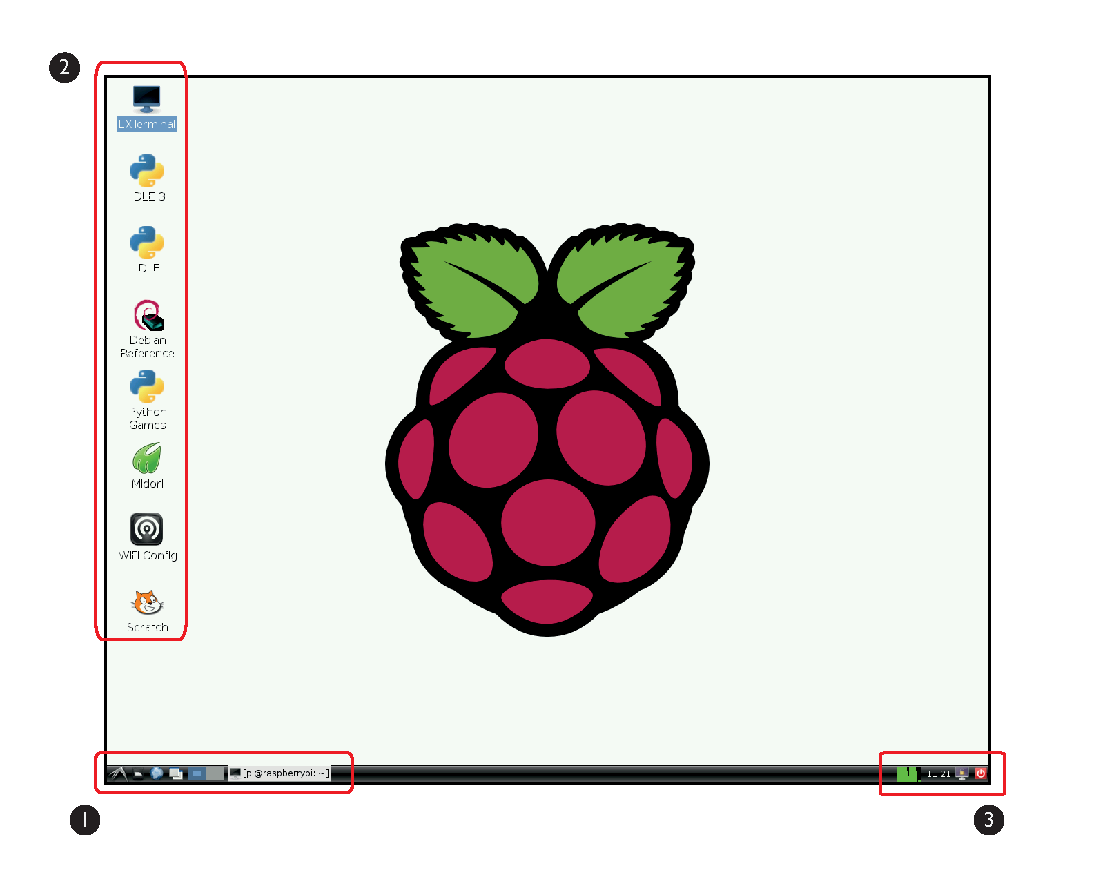
\includegraphics[width=14cm]{images/lxde-desktop}}
\caption{The Pi's default window manager is called LXDE.}\label{figure:lxde-desktop}
\end{figure}

\section{Configure mutt}

Once you've found your way around LXDE, fire up a terminal so that you can configure your Pi to read your University email using \cmnd{mutt}{Mutt}. Unlike the lab machines, \cmnd{mutt}{Mutt} isn't installed by default on the Pi, so you'll need to do that yourself using:

\begin{ttoutenv}
$ sudo apt-get install mutt
\end{ttoutenv}

Once the install has completed, you'll need to adjust Mutt's settings so that they once again point at your University email account. You could do this by following the instructions in the previous session's script again, but there's a much easier way: let's just copy the configuration file you created on the desktop PC last time, over to the Pi. 

First you need to check that you still have the \fname{.muttrc} configuration file in your home filestore of your Computer Science network account. You \textit{could} unplug all the cables from the Pi, connect them back into the desktop PC and check that way, but that's no fun (especially because we'd then have to reverse it all to do the next bit of the exercise). But you don't need to do that--you can check \concept{remotely}. 

\begin{note}
Picture of the hostname sticker, and update this with new new hostname style
\end{note}

So, find the hostname of the lab PC on your desk; there should be a sticker on both the PC itself and the monitor with a name such as `E-C07KILF3101'. If for some reason there isn't a sticker, there are several ways you can find out the hostname (you'll need to switch the monitor back to the DisplayPort input, and may also need to re-attach the keyboard/mouse usb lead to the desktop PC):

\begin{itemize}
\item If you haven't logged into the PC, then it should be showing a login prompt like  \ttout{E-C07KILF3101:}
\item If you're already logged in, but have not started a window manager, your console prompt will be something like  \verb|[mrnoodle@E-C07KILF3101 ~]$| (where \ttout{mrnoodle} would be replaced by your own username, of course).
\item If you are logged in to the PC and inside a window manager, open a terminal window. It should show you the command line prompt, as above. You could also type \verb|echo $HOSTNAME|.
\end{itemize}

Once you've got hold of the PC's hostname, we're going to use a \wikipedia{Secure_Shell}{Secure Shell} to connect to from the Pi to the the desktop, allowing you to type commands on the Pi that will be executed remotely via a shell that's executing on the desktop PC. In the terminal window on the Pi, issue this command:

\begin{ttoutenv}
$ ssh [USERNAME]@[HOSTNAME].cs.man.ac.uk
\end{ttoutenv}

replacing [USERNAME] with your University username, and [HOSTNAME] with the name of the PC in front of you. You'll need to enter your University password, and will most likely be presented with text something similar to this:

\begin{ttoutenv}
The authenticity of host 'E-C07KILF3101 (130.88.197.112)' can't be established.
RSA key fingerprint is 20:6d:2d:90:5e:8f:9f:19:39:70:ce:48:a6:93:ec:4c.
Are you sure you want to continue connecting (yes/no)? 
\end{ttoutenv}

Type \ttout{yes} (and hit enter) in response to the question. You should then be given a command prompt (you'll learn more about what this message actually means in \courseunit{COMP18112}, but for now just treat it as something that happens the first time you try to connect to a particular machine). Notice that this command prompt no longer says \ttout{pi@raspberrypi}, but rather has the name of the machine you've just remotely logged into. 

Type \cmnd{ls}{ls -a} to confirm that your \fname{.muttrc} file is still where you expect it to be, and if all is well then press \ctrl{D} to log out of the remote shell you just started, and you will return to the shell running locally on your Pi (you'll see the command prompt change back to being `pi' again). Now we know the file we want is there, we need to copy it from your Computer Science filestore onto your Pi's local filestore.

To do this, we're going to use the \cmnd{scp}{scp} (Secure Copy) command, which in some ways behaves like \cmnd{cp}{cp}, but allows us to move files \textit{between machines}. 

Like \cmnd{cp}{cp}, the \cmnd{scp}{scp} command in its basic form takes two arguments, the first is the name of the source file (the one you want to copy), and the second is the name of the destination file (the one you want to create). The difference with \cmnd{scp}{scp} is that either (or less commonly, both) of these files can be on a remote machine, which means that you need to provide the command with enough information about the location of the remote file in terms of the hostname and file system, and any login details necessary to get at it. The syntax for providing this information is:

\begin{ttoutenv}
[USERNAME]@[HOSTNAME]:[FILEPATH]
\end{ttoutenv}

So for example, if you wanted to retrieve a file called \fname{cheese.jpg} from the home directory of a user called \ttout{mrnoodle} that was stored on a machine with the hostname \ttout{mypc.example.com}, and you wanted the local copy of the file to be called \fname{mycheese.jpg} the command would be:

\begin{ttoutenv}
$ scp mrnoodle@mypc.example.com:cheese.jpg mycheese.jpg
\end{ttoutenv}

Then, supposing you had edited the file \fname{mycheese.jpg} on your local machine and wanted to put the file back into the home directory of the \ttout{mrnoodle} account on the remote machine, but under a different name (so as not to over-write the original), you would use the command:

\begin{ttoutenv}
$ scp mycheese.jpg mrnoodle@mypc.example.com:newcheese.jpg
\end{ttoutenv}

We're not exactly sure why MrNoodle and cheese feature quite so prominently in these labs either, just go with the flow. Now use your new-found knowledge of \cmnd{scp}{scp} to copy the \fname{.muttrc} file from your Computer Science account onto your Pi. Conveniently, there's nothing in the \fname{.muttrc} file that is specific to the Computer Science account setup, so you can use it as-is for Mutt on the Pi (as usual, if you get stuck as for help.)

Check that the file has copied over successfully using \cmnd{less}{less}, and then start up \cmnd{mutt}{Mutt} from a terminal. If everything has gone to plan, you should now be able to read and compose emails on your Pi. You can of course install other mail clients if you want to; there is a version of Thunderbird for the Pi called Icedove (yes, yet another play on words), or a much leaner graphical client called Claws Mail (which if you want to can be installed using \ttout{sudo apt-get install claws-mail}). Remember, though, that the memory-card we've given you for your Pi is fairly small, so you probably don't want to clutter it up with unnecessary packages, and you should find that Mutt is perfectly okay for sending and reading the occasional email. 

\subsection{Emailing your tutor}

To test that you've sucessfully set \cmnd{mutt}{mutt} up on the Pi, use it to send a friendly email to your tutor to tell him or her that you're reached this point of the lab . If you've not figured out your tutor's email address yet, you can find it at
\\
\url{http://www.cs.manchester.ac.uk/aboutus/people/}

\section{X Windows again}

As we mentioned before, the X Windows system is a powerful beast, and although it was designed a long time ago (around 1984), it was in many ways way ahead of its time--rather like the design of Unix itself.

Remember that the GUI you're now using on the Pi consists of two systems working together: X Windows (which amongst other things gives software access to the display hardware), and the Window Manager (in this case, LXDE) that provides the WIMP-style features such as movable windows and clickable controls. The X Windows system operates as a Client/Server architecture, where the `server' part does the drawing of stuff onto the screen, and clients request that things be drawn. One of the really nice features of X Windows is that it doesn't care too much about where the requests to draw things come from. Typically they come from processes that are running on the same computer as the X Server, but this need not be the case as you're about to demonstrate.

Log back in to the lab PC using the \cmnd{cmnd}{ssh} command, but this time include a \texttt{-X} switch before your username, like:

\begin{ttoutenv}
$ ssh -X [USERNAME]@[HOSTNAME]
\end{ttoutenv}

The \ttout{-X} switch (note that it's an uppercase X) tells the \cmnd{ssh}{ssh} program to send any X Windows graphics generated on the remote generates back through the network from the remote machine to the X Server running on the local machine.

\begin{note}
Fix / simplify the above
\end{note}

Confirm that you are indeed logged into your Computer Science account by checking the command prompt and using \cmnd{ls}{ls} to make sure the files in your home directory are the ones you'd expect, and then type:

\begin{ttoutenv}
$ xeyes
\end{ttoutenv}

Googly eyes that follow the mouse! What's not to like? Well, okay, perhaps not hugely exciting in itself, but what's actually happening here is rather interesting and quite sophisticated. The \cmnd{xeyes}{xeyes} program is running on the remote machine (the desktop PC); but the instructions to draw its graphical output are being forwarded over the secure shell connection you've made from the Pi to the remote machine, so that the Pi's X Windows system receives them. Press \ctrl{C} to quit \cmnd{xeyes}{xeyes}, and instead try running \cmnd{xterm}{xterm}. You should see a new terminal window appear on your Pi's screen (which probably looks slightly different to the terminal you launched on the Pi a moment ago; it does essentially the same thing though). This X Terminal, rather like \cmnd{xeyes}{xeyes}, is actually running on the desktop machine---only its graphical representation is appearing on your Pi (if you use \cmnd{ls}{ls} in that terminal, you'll see that its your Computer Science account that's visible, rather than your Pi's filestore and you can confirm this another way using the \cmnd{hostname}{hostname} command). 

%How could you use this feature to your advantage to give you a temporary graphical mail client (or perhaps to use Firefox as a web browser, rather than Midori) on the Pi without needing to install any packages on the Pi itself? 

\begin{note}
may need a diagram to help explain what's going on here
\end{note}

\section{A Simple Web Server}

This next exercise involves setting up a simple web server on the Pi, but before we can do that you'll need to create some basic web pages to display. 

\begin{note}
fix this bit
\end{note}

Start up a terminal, and use the \cmnd{mkdir}{mkdir} to create a directory called \ref{FIXME} your home directory, and in that directory, use \cmnd{nano}{nano} to create a file called \fname{index.html} with the following content:

\begin{ttoutenv}
<html>
<body>
Hello world!
</body>
</html>
\end{ttoutenv}

From within that directory, run the command:

\begin{ttoutenv}
$ python -m SimpleHTTPServer
\end{ttoutenv}

and then use Midori to browse to the following URL:

\begin{ttoutenv}
http://localhost:8000
\end{ttoutenv}

If your browser displays a page saying `Hello World', pat yourself on the back---you've just created a web page \textit{and} set up a simple web server to host it. The URL you used to view this page may look a bit odd compared with others you have seen. The \texttt{http://} part you'll no-doubt be familiar with from other web-addresses that you've seen; the `localhost' part is a convention that means `this machine'. The section of the URL that follows \texttt{localhost} may be even less familiar: this is the \textit{port} (communication channel) on which the simple web-server that you've set up is serving web pages; by default web browsers expect servers to use port 80, but the \ttout{python -m SimpleHTTPServer} command you used here defaults to port 8000, so we had to add that to the URL. We'll leave the issue of ports there for now, and revisit that in more detail in the 2nd semester in \courseunit{COMP18112}. 

\subsection{A slightly more interesting web page}

\begin{note}
give them a default MrNoodle Webpage
\end{note}

Now spend a few minutes modifying \fname{index.html} to create a slightly more interesting web page. Create a single page about yourself that contains a paragraph describing who you are, which programme you're on (e.g. Computer Science, Software Engineering, etc.), and which contains a picture of yourself as well as the image you created in the previous session using Inkscape.

Don't worry about finely crafted words here---this is really just a way of creating a file that we can get you to edit in various ways a little later on. A few sentences will do, and you can always change it later. 

As for the photograph of you, we'd ideally like you to use something recent that someone could recognise you by, but it doesn't really matter too much: it can be any kind of photo you like; silly or serious, whatever you're comfortable with, but please make sure it doesn't contain anything offensive. If you're not comfortable with having a photo of yourself on the net, you can use a photo of something else (but you must make sure you have permission to re-use a picture that's not yours; anything you find on Wikipedia should be okay for this purpose, and there will be more guidance on how to use others' photos later in this course). If you didn't have a photo handy, take one with your phone, or ask one of your fellow students to do it for you on theirs.

You've already learned several ways of getting files onto your Pi, but here's a reminder:
\begin{itemize}
\item You could mail the photo to yourself, and use Mutt to save the attachment onto the Pi (more help on how to do this in Breakout~\ref{breakout:attachments})
\item If the picture is on the web somewhere, you could use Midori to find and save it. 
\item Alternatively for images on the web, you could use \ttout{curl} to fetch it directly from a URL to a file. 
\item You could use \ttout{scp} to copy it from some other machine directly to your Pi. 
\item Or if all else fails, you could use a USB device to copy it from one place to another. 
\end{itemize}

\begin{diversion}{Saving attachments with Mutt}
\label{breakout:attachments}
splunge
\end{diversion}

If you need more guidance on how to write the web page itself, then Appendix~\ref{appendix:simplehtml} contains a few pointers; though there are plenty of tutorials on the web as well. 

To finish this section, use Midori to check that your web page is displaying correctly.

\section{Headless Pi}
\label{section:headless}



\begin{note}
put a warning in here that it's a bit scary and we'll come back to it later.
\end{note}



The Pi can be used as a respectable desktop machine, but it really comes into its own as a `server' or controller for other pieces of hardware. In this section we'll use the Pi in what is called `headless' mode, that is without its own screen and keyboard, to create a proper web server to host your pages. 

At a terminal, type the command \ttout{ifconfig}, short for `interface configuration', which will give you details about the network configuration on the Pi. This will return something along the lines of

\begin{ttoutenv}
eth0      Link encap:Ethernet  HWaddr b8:27:eb:a5:d5:82
          inet addr:10.2.215.1  Bcast:10.2.215.255  Mask:255.255.255.0
          UP BROADCAST RUNNING MULTICAST  MTU:1500  Metric:1
          RX packets:39778 errors:0 dropped:0 overruns:0 frame:0
          TX packets:4338 errors:0 dropped:0 overruns:0 carrier:0
          collisions:0 txqueuelen:1000
          RX bytes:18251497 (17.4 MiB)  TX bytes:651537 (636.2 KiB)

lo        Link encap:Local Loopback
          inet addr:127.0.0.1  Mask:255.0.0.0
          UP LOOPBACK RUNNING  MTU:16436  Metric:1
          RX packets:105 errors:0 dropped:0 overruns:0 frame:0
          TX packets:105 errors:0 dropped:0 overruns:0 carrier:0
          collisions:0 txqueuelen:0
          RX bytes:8550 (8.3 KiB)  TX bytes:8550 (8.3 KiB)
\end{ttoutenv}

This tells you that the Pi has two network devices currently active: one called `eth0', which is the represents the physical ethernet socket into which you plugged the blue network cable, and which allows the Pi to communicate with other computers on the network (and in this case, on the internet); and a second one called `lo' which is a `virtual connection' or `local loopback' connection that allows the Pi to route network traffic back to itself (this is how the `localhost' trick you used earlier to look at web pages on the Pi worked). You'll learn a lot more about network configuration in the second year Computer Networks course (COMP28411). 

The thing we're interested in right now is the IP Address that's been allocated to your Pi. Look for the line in the \texttt{eth0} block of text that says \texttt{inet addr:} and note down the number that follows this in your logbook (in the case of our example that is 10.2.215.1 but in your case it will probably be something else). Don't worry too much about what this number means or where it came from for now---we'll return to this in \courseunit{COMP18112} in the second semester. For now, just treat this as being a unique number that identifies your Pi on the Computer Science network. 

Quit the graphical environment, and log out of your Pi. Leave the network connection and power supply plugged in, but disconnect the mouse/keyboard lead, and reconnect them to the desktop PC. Switch the monitor over to display the desktop PC's screen, and log in to that with your University credentials. 

Once you're in the graphical window environment, start up a terminal, and use \cmnd{ssh}{ssh} to log into your Pi:

\begin{ttoutenv}
$ ssh pi@[IPADDRESSOFPI]
\end{ttoutenv}

replacing [IPADDRESSOFPI] with the IP Address you noted down a moment ago. Since this is the first time you're logging in from your CS account to your Pi, expect to see the `The authenticity of host' warning again; just say `yes' to the prompt, and enter your Pi user's password. 

Change directory to the `aboutme' directory you created for your web-page earlier, and re-start the simple Python web server. 

Next, start up Firefox using the keyboard shortcut you created in the previous lab session, and enter the URL:

\begin{ttoutenv}
http://[IPADDRESSOFPI]:8000
\end{ttoutenv}

and you should see your web page appear, served off your Pi to the desktop machine just like a real web server. Get the person next to you to see if they can see your web page from their machine by using your Pi's address; and return the favour by checking that theirs is also working (it's worth noting that the IP addresses of the Pis are only visible within the School of Computer Science, so pages served off your Pi will not be visible on the wider Internet).


\subsection{Setting up Apache, a proper web server}

The simple Python-based web server that you've been running so far is doing the bare minimum necessary to allow HTML pages to be fetched by a browser. Although it was a handy way of getting you going with web server technology, it's a long way off being the kind of fully-featured web server you would need to run a modern website. Fortunately, the Apache HTTP Server---the software that \textit{is} used to run over half the world's websites---is Open Source and runs quite happily on a Raspberry Pi. You wouldn't want to be powering the next eBay or Facebook from a Pi, but to illustrate the principles, it'll do the job nicely. 

Before we install Apache on your Pi, there's a bit of housekeeping to do that will conveniently expose you to a few more Unix concepts that we've rather skated over so far. 

\subsection{Permissions, users and groups}

Right at the beginning of these sessions you logged in to the Pi as a particular user called `pi', and on the desktop machines you've been logging in using your University username and password. It's fairly obvious what the general principles are here---logging in with a username and password is a way of protecting `your stuff' from being seen or messed around with by other users. Roughly speaking this means two things: first, and most obviously, files created by you should be in some sense `owned' by you so that you can control who can see/modify them; second, and perhaps less obviously, processes that you start---whether from the command line or the graphical environment---are also `yours' and have certain privileges/restrictions that are associated with your user. 

For this to work, it means that both the Unix file system and its way of dealing with processes need to be aware of the notion of a user. Back in the terminal that's connected by \cmnd{ssh} to your Pi, use \cmnd{cd}{cd} to change to your home directory and issue \cmnd{ls}{ls -l} to list the files there in what's called `long format' (the \ttout{-l} switch means `give me extra information about each file'). You'll see something like Figure \ref{figure:longformls} (but without the coloured background, which we've added to help distinguish the different columns in the figure).

\begin{figure}
\centerline{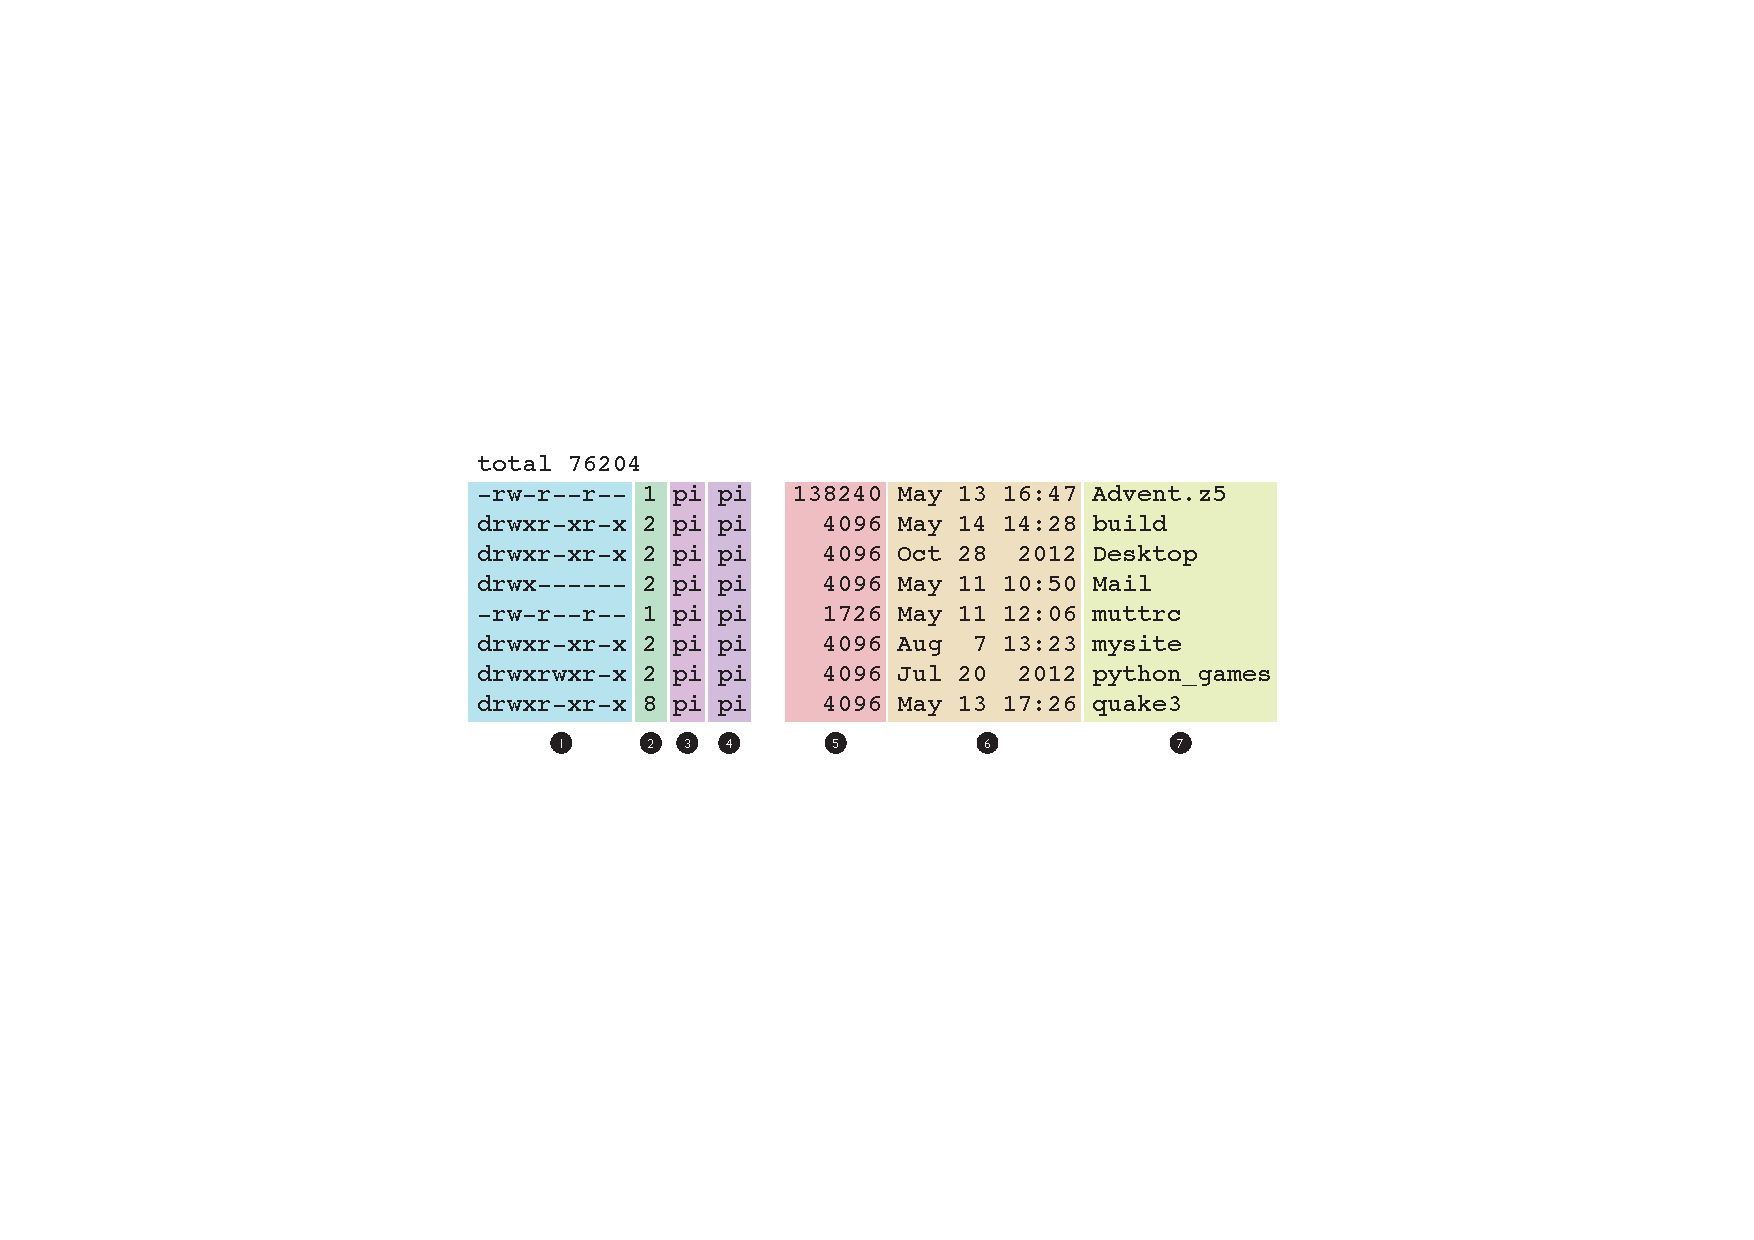
\includegraphics[width=14cm]{images/longformls}}
\caption{An example of the `long format' output from ls.}\label{figure:longformls}
\end{figure}

Working from right to left in Figure \ref{figure:longformls}, column \protect\circled{7} contains the filename, column \protect\circled{6} gives the date that the file was last modified (the exact format of the date will vary so as to always be `useful'; older files will have a year instead of an exact time, for example) and column \protect\circled{5} shows the size of the file in bytes. Columns \protect\circled{4} and \protect\circled{3} give the group and user to which the file belongs (often these will appear to be the same name); we'll come back to this in a moment. Column \protect\circled{2} shows the number of links associated with the file (ignore this for now), and finally column \protect\circled{1} gives a summary of the file's permissions, which we'll look at again shortly. 

In our example, the file's user (Column \protect\circled{3}) is not surprisingly `pi', which is the username under which you logged in. Run 

\begin{ttoutenv}
$ ls -l /
\end{ttoutenv}

(i.e. `long format list of the root directory), and you'll see that the files at the top of the filesystem are owned by a user called \ttout{root}. 

As well as being owned by a particular user, each file is associated with a \textit{group} (shown in column \protect\circled{4}, which in this case is a group called `pi' too; although both the user and the group are called pi here, they are different things). Every user is a member of one or more groups. The idea of a Unix group is quite straightforward: it's a mechanism to allow collections of users to share resources with one another in a controlled way, while stopping other unwanted users from being able to access those resources. For example, you might want to say ``Only I as this file's creator am allowed to modify or delete this file, but other members of my Tutorial Group can read the file's content, and the file is inaccessible to everybody else''. In Unix each file can have three different types of access permission: read, write and execute (run). These permissions can be set for three different categories of user: user (`owner'), group (a specific set of users) and `other' (which means `everyone else').

The file permissions shown in column \protect\circled{1} of Figure \ref{figure:longformls} consist of 10 `slots' as shown in more detail in Figure \ref{figure:fileperms}. The first slot indicates the type of the file, and appears as a \ttout{-} for a regular file or a \ttout{d} for a directory. The next three slots represent the \concept{user}'s  permissions and can consist of any combination of \ttout{r} for `readable', \ttout{w} for writable and \ttout{x} for executable. The next three slots show the read/write/execute permissions for members of the file's \concept{group}, and the last three slots show the same set of available permissions for \concept{other} (i.e. anyone else with access to the system). Execute permissions when applied to a directory mean that particular set of users can access the directory's contents.

\begin{figure}
\centerline{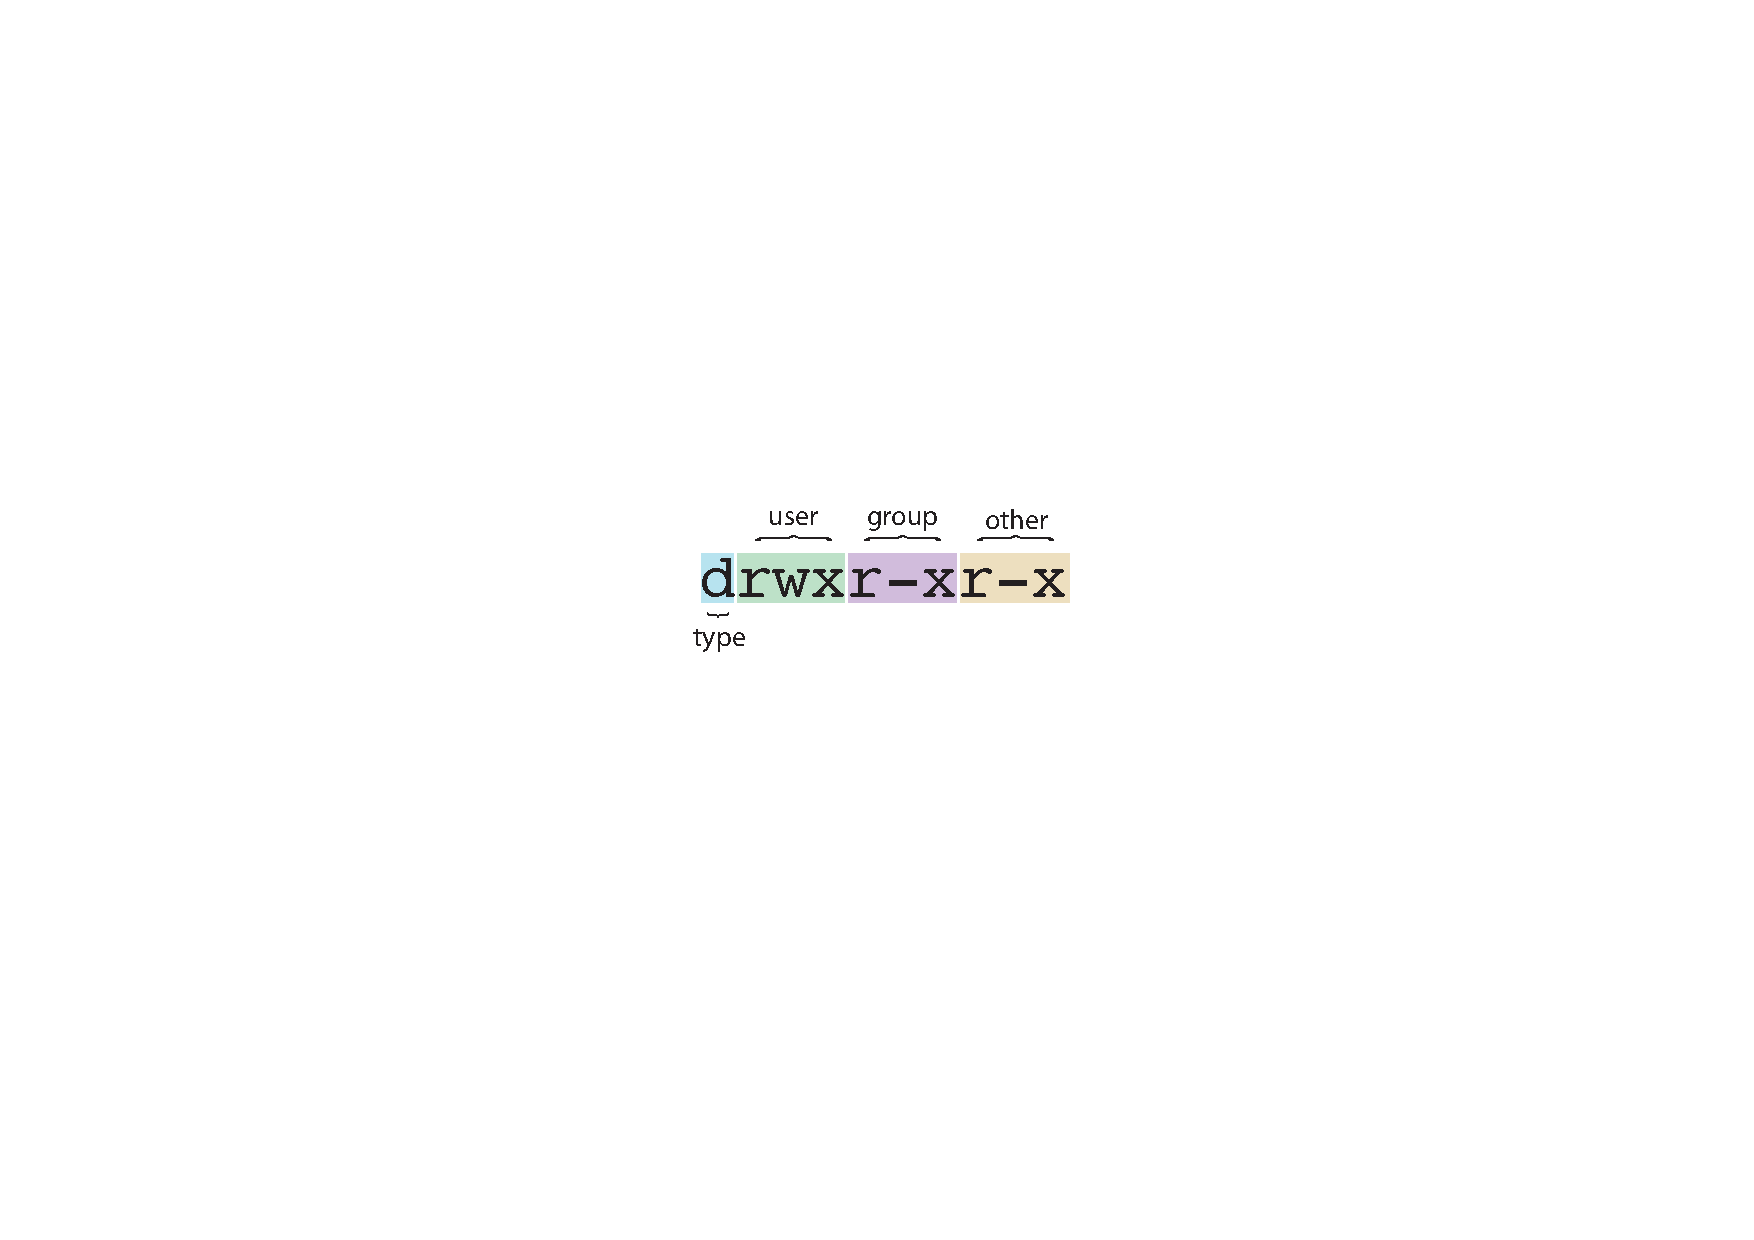
\includegraphics[width=7cm]{images/filepermissions}}
\caption{Unix file permissions as shown with \ttout{ls -l}. In this example shows the permissions for a directory that can be read from, written to and listed by its user (owner), but only read and accesed by group members or anyone else.}\label{figure:fileperms}
\end{figure}

We'll come back to file permissions in more detail shortly. In the meantime, let's look at the ownership model for processes. Type:

\begin{ttoutenv}
$ ps waux
\end{ttoutenv}
% $

to list any processes that are currently running (you'll probably need to widen the terminal window to see the output properly). The \cmnd{ps}{ps} command is unusual in that if used with no arguments, its output is largely uninformative. It's also unusual in that explaining what even the most basic arguments do and interact (i.e. the \ttout{waux} options in this case; note that there's no hyphen in front of the options here), is quite complex---so for now just treat this as a special recipe that does something useful. 

Look at the rightmost column of the output (which has the heading `COMMAND') and you should see a few familiar process names such as bash, \cmnd{startx}{startx}, and the \cmnd{ps}{ps} process itself in amongst many commands that will be unfamiliar to you at the moment. The rightmost column tells you who owns the processes, and you'll see that the majority of them are owned by you (or, rather by the user `pi'), and a small number of them are owned by the root user. Most of the processes that you're seeing have been started as part of the window manager system, or are in one way or another associated with X Windows; the rest are `housekeeping' processes the details of which we don't care about for now. 

If you think back to what you learned about the hierarchical relationship between processes in the first Pi lab, it should be starting to become clear how the `family tree' of processes when combined with the notion of users and resource ownership knit together nicely to give a secure multi-user system. When you first log in to a Unix machine, a single process is started on your user's behalf (in most cases this is a command shell). From that shell you can start other processes, which could be individual commands like \ttout{tar} or \ttout{ls}, or could be a whole window manager system such as Gnome or LXDE; in either case though, these inherit the properties of the parent shell in terms of being owned by the same user. Then, any processes that are started by the window manager also inherit the same user properties, and so forth. 

\subsection{Back to that webserver}

Anyway, let's get back to setting up the Apache web server. When you ran the python web server, that was a process owned by you, and because we didn't do anything special to protect it, if you closed the shell/terminal that was used to start it, it too would die. Generally speaking, you'd want a web server to continue running whether anyone was logged into the machine or not, so this isn't ideal. The other issue with starting a web server in this way is that because the process is owned by you, it has access to all your files---so if a malicious hacker was able to take control of the web server process, he or she would be able to read or even delete your work, which clearly isn't a good thing. 

So to set up a web server properly we need to

\begin{itemize}
\item make sure that it can continue to function after you've logged out, and
\item somehow make sure that it can only access a specific set of resources that represent the website, and not run riot around your filestore doing bad things. 
\end{itemize}

Let's first tackle the issue of a shared directory; this is quite easy to set up using Unix's group mechanism. 

By default, the Apache package that we're going to install shortly is set up to serve web pages from a directory called \fname{/var/www} and although you can change it in Apache's configuration files to be elsewhere, that's as good a place as any for what we need. 

Let's go ahead and install Apache using the command:

\begin{ttoutenv}
$ sudo apt-get install apache2
\end{ttoutenv}

It's a reasonably large package so may take a little while to install; just be patient. Once that's completed, take a look in \fname{/var} using \ttout{ls -l} and you should see a directory in there called \fname{www} which is owned by root.

Before we start serving any web pages, there are a few security issues that we need to take into account. In its simplest form, where you're just serving static web pages (i.e. HTML files), Apache is secure enough, but as soon as you start creating web sites where users can add and modify content on your server, you potentially open yourself up to malicious damage, so it's best to take some initial precautions. 

Take a look at the permissions for \fname{/var/www}, which was created when you installed the Apache package, and you will see that they are set to \ttout{drwxr-xr-x} which means `this is a directory that the owner can read, write and access the contents of, and which both group and other users can only read and access'. Notice too that there's a single file in that directory called \fname{index.html}, which is an `it works!' declaration that you can use to test that Apache is doing the right thing (and which we'll do shortly). The important thing here is that anybody or any process that is not running as the root user has only got \concept{read} and not \concept{write} access to the contents of the \fname{/var/www} directory structure---and this is exactly what we want. They can look, but not touch, and so can't break anything. 

But how do we get content into the \fname{/var/www} directory so that it can be served by Apache? We could simply use \fname{sudo} to give ourselves root privilege every time we need to modify a file, but that's a rather clumsy solution: we may not want other users on our machine to have root access at all, and in any case you really do want to keep sudo commands to a minimum so that you don't accidentally do something bad to your system. So let's create a new group that will represent users on the Pi that are allowed to put content into that directory. Use the command \cmnd{addgroup}{addgroup} to create a new group called \ttout{www-contrib} (for `web contributors'). The syntax is straightforward:

\begin{ttoutenv}
$ sudo addgroup www-contrib
\end{ttoutenv}

And you should see that a new group has been created with a Group Identifier (GID) probably set to 1001. 

Change the group ownership of \fname{/var/www} to be \ttout{www-contrib} using the command

\begin{ttoutenv}
$ chgrp -R www-contrib /var/www
\end{ttoutenv}

and check that this has changed using \ttout{ls -l}. Note that we're using the \ttout{-R} option to \cmnd{chgrp}{chgrp}, which means `apply this change not only to /var/www itself, but to all files and directories contained within it' (`R' here stands for \wikipedia{Recursion}{recursive}). Next we need to add the pi user to that group. Type

\begin{ttoutenv}
$ groups
\end{ttoutenv}

to see what groups your user is already a member of (you'll see things like \ttout{pi}, \ttout{adm}, \ttout{dialout}, \ttout{cdrom}, \ttout{sudo} and several others). Use the command 

\begin{ttoutenv}
$ sudo usermod -a -G www-contrib pi
\end{ttoutenv}

to add the Pi user to the www-contrib group. The \ttout{usermod} command can be used to modify lots of things about a user; here we are using with the combination of \ttout{-a} and \ttout{-G} to mean `append this group to the user's list of groups'. You'll need to log out and back in again to see this change take effect, so do that now and then run the \ttout{groups} command to confirm that pi is now indeed a member of group \ttout{www-contrib} as well as the other original groups. 

\begin{diversion}{About groups}
\label{diversion:aboutgroups}
Explain what the other groups are for
\end{diversion}

We now need to make the \fname{/var/www} folder \textit{writable} by members of our new group, so do that using the command

\begin{ttoutenv}
$ sudo chmod -R g+w /var/www
\end{ttoutenv}

which reads as `modify the permissions of the directory /var/www and any files/directories in it to add write access for members of its group'. 

Now if all has gone to plan, the user pi should be able to read and write to the directory \fname{/var/www}. Try this out by editing the content of the \fname{index.html} file that's in that directory (and which was created when you installed Apache) to say something different from the default text.

We're finally ready to start Apache. Use the Apache Control command

\begin{ttoutenv}
$ sudo apachectl start
\end{ttoutenv}

to initialise the server (you can use a similar command with `stop' to shut it down again), and then use \cmnd{ps}{ps waux} to confirm that you can see several processes with `apache' in the name now running. Note that although you started the server with \cmnd{sudo}{sudo} which runs things as root, that the owner of the apache processes is \fname{www-data}. The \ttout{apachectl} command has restricted apache to running as a regular, non-root user, and you should by now be able to work out why having a web server running as root would be a Bad Thing from a security point of view.

On the desktop machine use a web browser to see what content the Pi is now serving. The URL will be 

\begin{ttoutenv}
http://[IPADDRESSOFPI]
\end{ttoutenv}

and since we're now using a standard web server on a standard port, there's no need to add the :8000 port number as we did in Section \ref{section:headless}. 

You should see the `It works!' page appear, with whatever modification you made to it a moment ago.

Finally for this lab session, copy the content from your `aboutme' directory so that its served via Apache.  

\begin{note}
COPY OVER TO DESKTOP MACHINE, HALT THE PI and restore the desktop
\end{note}


\chapter{Using Linux in CS}

\begin{note}
  This is where the script for the third, two hour lab, should go
\end{note}



\end{document}
                                
%%% Local Variables: 
%%% mode: latex
%%% TeX-master: t
%%% End: 
